\chapter{Magnetoest'atica}


\section{Corriente y densidad de corriente}

Cuando existen cargas en movimiento, se define la \textit{corriente el'ectrica} $I$ como
la cantidad de \textit{carga neta} que pasa por unidad de tiempo a trav'es de una superficie $S$ \textit{en una direcci'on determinada}, 
\begin{equation}\marginnote{Corriente el'ectrica}
I(t) :=\lim_{\Delta t\to 0}\frac{\Delta Q}{\Delta t}=\frac{dQ}{dt},
\end{equation}
de modo que la carga neta que atraviesa entre los tiempos $t_1$ y $t_2$ una superficie por donde circula una corriente $I(t)$ es
\begin{equation}
Q=\int_{t_1}^{t_2}I(t)\,dt.
\end{equation}
La unidad S.I. para la corriente es el \textbf{Amp\`ere}: $1A:=1C/1s$.

\subsection{Densidad de Corriente}

Consideremos una superficie sobre la cual inciden cargas con densidad $\rho$,
movi'endose con velocidad $\vec{v}$, cruzando un elemento de superficie (orientado) $d\vec{S}$.
\begin{figure}[!h]
\centerline{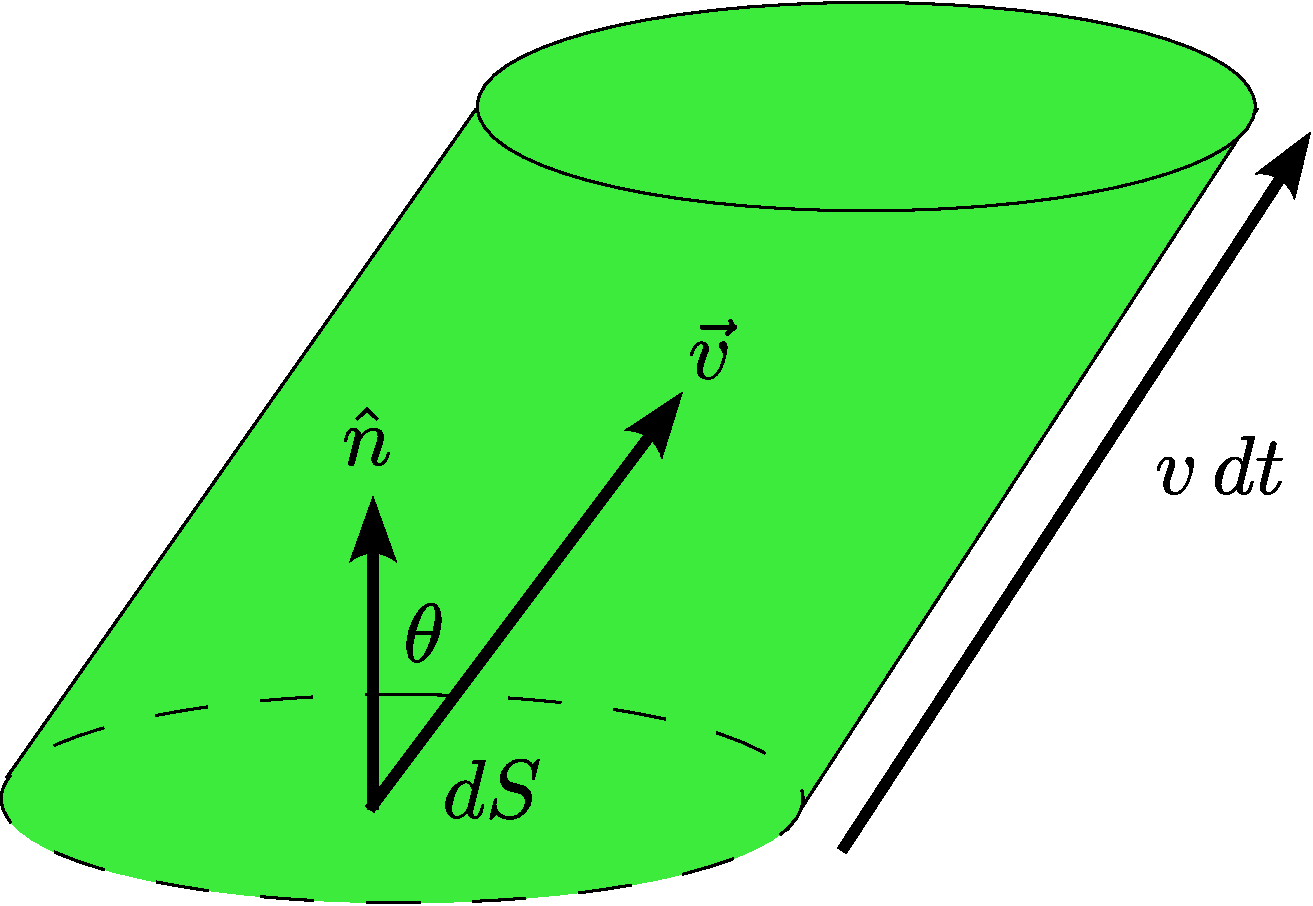
\psfig{file=fig/fig-flujo-cargas-01.pdf,height=4cm,angle=0}}
\caption{Carga con densidad $\rho$ flujendo con velocidad $\vec{v}$ a trav'es
de un elemento de superficie $d\vec{S}$.}
\label{MD1}
\end{figure}
La carga neta que atraviesa el 'area $dS$ en un intervalo de tiempo $dt$ es la que
est'a contenida en un cilindro oblicuo de base $dS$ y de largo $v\,dt$. Ver
figura \ref{MD1}.

Esto permite escribir:
\begin{equation}
dQ=\rho\, dV=\rho\, dS\,(v\,dt)\cos\theta=\rho\,\vec{v}\cdot d\vec{S}\,dt.
\end{equation}
Definimos la \textbf{densidad de corriente}
\begin{equation}\marginnote{Densidad de Corriente}
\boxed{\vec{J}(x):=\rho(x)\vec{v}(x),}
\end{equation}
de modo que
\begin{equation}
 dQ=\vec{J}\cdot d\vec{S}\,dt .
\end{equation}
En otras palabras, la densidad de corriente es la carga por unidad de tiempo y
por unidad de superficie que atraviesa un elemento de 'area normal dado.
Como consecuencia, la corriente, es decir, la carga por unidad de tiempo,
que atraviesa una superficie $S$ es dada por
\begin{equation}
I=\int_{S}\vec{J}\cdot d\vec{S}.
\end{equation}
Es importante notar que si $\rho>0$, entonces $\vec{J}$ y $\vec{v}$ tienen igual
sentido, mientras que si $\rho<0$, entonces $\vec{J}$ y $\vec{v}$ tienen
sentidos opuestos.

\section{Conservaci'on de la carga el'ectrica}

La ley (experimental) de conservaci'on (local) de la carga el'ectrica puede ser escrita
en general, como
\begin{equation}
\frac{d{\ }}{dt}\int_V \rho\,dV=-\int_{\partial V}\vec{J}\cdot d\vec{S},
\end{equation}
que expresa el hecho que todo cambio en la carga neta contenida en un volumen $V$ dado (pero arbitrario) es debido al flujo neto de carga por la superficie ${\partial V}$ que lo encierra. Usando el teorema de Gauss, podemos transformar la integral de superficie a una integral de volumen, obteniendo
\begin{equation}
\int_V\left(\frac{\partial\rho}{\partial t}+\vec{\nabla}\cdot\vec{J}\right)\,dV
 =0.
\end{equation}
Como esta relaci'on debe ser v'alida para todo volumen $V$, es decir, de tama\~no y forma arbitraria, es necesario que
\begin{equation}\marginnote{Conservaci'on local carga}
\boxed{\frac{\partial\rho}{\partial t}
+\vec{\nabla}\cdot\vec{J}=0.}\label{eccont}
\end{equation}
Esta relaci'on es conocida como la \textit{ecuaci'on de continuidad}.

\subsection{Corrientes Estacionarias}

Un caso de particular inter'es es aquel en que las corrientes son
\textit{estacionarias}, es decir, en las que tanto $\rho$ como $\vec{J}$ \textit{no dependen del tiempo}. Bajo estas condiciones, la ecuaci'on de continuidad requiere que la
divergencia de la densidad de corriente sea nula:
\begin{equation}\marginnote{Caso estacionario}
 \vec{\nabla}\cdot\vec{J}=0. \label{divJ0}
\end{equation}


% \subsection{Modelo de Conductividad}
%
% Suponemos que los electrones se mueven en la red at'omica. La ecuaci'on
% de movimiento es
% \begin{equation}
% mn\frac{du_i}{dt} -nqE_i=F_i%
% \label{magstatica-mov}%
% \end{equation}
% donde $T$ es la temperatura del gas de electrones, y $F_i=-mn\nu u_i$ es
% la fuerza debido a las colisiones. Recordando que $\rho=nq$ y que
% $j_i=nqu_i$ tenemos que en la ecuaci'on (\ref{eccont} )
% resulta%
% \begin{equation}
% \frac{\partial\rho}{\partial t}+\partial_i\left(  \rho u_i\right)  =0
% \end{equation}
% de la ecuaci'on (\ref{magstatica-mov}) y suponiendo que el gradiente de
% temperatura es despreciable, tenemos%
% \begin{align*}
% mn\frac{du_i}{dt}-nqE_i  & =-mn\nu u_i\\
% n\frac{d\left(  u_i\right)  }{dt}  & =\frac{nq}{m}E_i-\nu u_i%
% \qquad\qquad/\cdot q\\
% \frac{d\left(  nqu_i\right)  }{dt}  & =\frac{nq^2}{m}E_i-\nu nqu_i\\
% \frac{dj_i}{dt}+\nu j_i  & =\frac{nq^2}{m}E_i%
% \end{align*}
% Si $\vec{J}$ es constante en el tiempo%
% \begin{equation}
% j_i=\frac{nq^2}{m\nu}E_i=\sigma E_i%
% \end{equation}
% llamando a $\sigma$ conductividad el'ectrica. Notar que la conductividad es
% inverso a la resistencia el'ectrica, es decir, $\sigma=1/R~~\left[
% 1/\Omega\right]  $

% \subsubsection{Aplicaci'on: Velocidad de distribuci'on de la carga}
%
% Velocidad con que se distribuye la carga el'ectrica en un conductor con
% conductividad $\sigma$. Veamos que,%
% \begin{equation}
% j_i=\sigma E_i%
% \end{equation}
% luego en la euaci'on de continuidad (\ref{eccont} ) tenemos%
% \begin{align*}
% \frac{\partial\rho}{\partial t}+\vec{\nabla}\cdot\vec{J}  & =0\\
% \frac{\partial\rho}{\partial t}+\sigma\partial_iE_i  & =0\\
% \frac{\partial\rho}{\partial t}+\frac{\sigma}{\varepsilon_0}\rho & =0
% \end{align*}
% Esta ecuaci'on diferencial tiene como soluci'on%
% \begin{equation}
% \rho(t)=\rho_0~e^{-t/t_0}%
% \end{equation}
% donde $t_0=\varepsilon_0/\sigma$. Para valores experimentales tenemos que
% $\varepsilon_0=8.8512\times10^{-12}~\left[  c^2/Nm^2\right]  $ y para el
% cobre se tiene que $\sigma=59.88~\left[  1/\Omega\right]  $ luego conociendo
% la densidad del cobre podemos saber como varia la densidad de carga en el
% tiempo para un volumen dado.

\section{Campo magn'etico y fuerza magn'etica}
Se ha encontrado \textit{experimentalmente} que la fuerza que act'ua sobre una peque\~na carga $q$, movi'endose con velocidad $\vec{v}$ en un campo magn'etico dado es proporcional a $q$, a la rapidez $v$, y que tiene direcci'on perpendicular a $\vec{v}$. Esto permite \textit{definir}  la \textit{intensidad de campo magn'etico} $\vec{B}$ como un (pseudo-)vector tal que (en el sistema internacional de unidades)
\begin{equation}
 \vec{F}_{\rm m}=q\,\vec{v}\times\vec{B}.
\end{equation}
Por lo tanto, la fuerza total que act'ua sobre una carga $q$ en un punto del espacio con campo el'ectrico $\vec{E}$ y magn'etico $\vec{B}$ es dada por la \textit{fuerza de Lorentz}\footnote{En honor a Hendrik Antoon Lorentz (1853-1928): f'isico y matem'atico holand'es. Ganador del Premio Nobel de F'isica en 1902. Ver \url{http://es.wikipedia.org/wiki/Hendrik_Lorentz}.}
\begin{equation}\marginnote{Fuerza de Lorentz}
\boxed{ \vec{F}=q\left(\vec{E}+\vec{v}\times\vec{B}\right).}
\end{equation}
La unidad de medida de la intensidad de campo magn'etico $\vec{B}$ es entonces  $[B]=Ns/Cm=Vs/m^2$ , que se define como un \textit{Tesla}: $1T:=Vs/m^2$. Alternativamente se define un
\textit{Gauss} como $1G:=10^{-4}T$. \footnote{Por ejemplo, la magnitud campo
magn'etico interestelar oscila entre $0,1$ and $10$ $nT$, el campo magn'etico
de la Tierra es de orden $\approx 0,5 G$, mientras que un im'an
de Neodimio (Nd${}_2$Fe${}_{14}$B) produce un campo del orden de $1.25\, T$.
Un magneto de un sistema de resonancia magn'etica produce campos entre $1,5\,T$
y $3\,T$. Los campos magn'eticos m'as intensos producidos en un laboratorio son
del orden de $100\,T$ \cite{MagLab2012,HZDR2011}. El campo magn'etico en una estrella de neutrones puede oscilar entre 1 y 100 MT.}

Como consecuencia directa del hecho que la fuerza magn'etica es perpendicular a
la velocidad de las cargas, \textit{el campo magn'etico no realiza trabajo} sobre ellas.
Esto tiene como consecuencia que el campo magn'etico s'olo puede cambiar la
direcci'on de la velocidad de una carga y no su m'odulo (energ'ia cin'etica).

Si las cargas est'an distribuidas continuamente, entonces la fuerza magn'etica total sobre una regi'on $V$ con densidad $\rho$ y velocidad $\vec{v}$ ser'a
\begin{equation}\marginnote{Fuerza magn'etica}
 \vec{F}_{\rm m}=\int_V
\rho\vec{v}\times\vec{B}\,dV=\int_V\vec{J}\times\vec{B}\,dV. \label{fm1}
\end{equation}
Podemos describir esta situaci'on usando la \textbf{densidad de fuerza
magn'etica} $\vec{f}_{\rm m}$, definida como la fuerza por unidad de volumen,
dada por
\begin{equation}
 \vec{f}_{\rm m}:=\vec{J}\times\vec{B},
\end{equation}
de modo que
 \begin{equation}
\vec{F}_{\rm m}=\int_V\vec{f}_{\rm m}\,dV. \label{dfm}
\end{equation}


% \subsection{Trayectorias en un campo el'ectromagn'etico}
% Usando () y la segunda ley de Newton, tenemos
% \begin{equation}
% m\frac{dv_i}{dt}=qE_i+q\varepsilon_{ijk}v_jB_k
% \end{equation}
% Multiplicando esta ecuaci'on con $v_i$, obtenemos
% \begin{equation}
%  \frac{d\ }{dt}(\frac{m}{2}v^2)=qv_iE_i
% \end{equation}
% \begin{equation}
%  \frac{dK}{dt}=qv_iE_i
% \end{equation}
% S'olo el campo el'ectrico realiza trabajo sobre la carga, modificando su
% energ'ia ci'n'etica.
% \begin{equation}
%  dK=qv_iE_idt=qE_idx_i=-q\partial_i\phi dx_i=-qd\phi
% \end{equation}
% \begin{equation}
%  d(K+q\phi)=0
% \end{equation}
% \begin{equation}
%  \frac{1}{2}mv^2+q\phi={\rm cte}
% \end{equation}
% a lo largo de la trayectoria.


\section{Ley de Biot-Savart}
Biot\footnote{Jean Baptiste Biot: F'isico, Astr'onomo y Matem'atico franc'es (1774-1862). Ver \url{http://es.wikipedia.org/wiki/Jean_Baptiste_Biot}.} y Savart\footnote{F'elix Savart: F'isico, M'edico y Profesor franc'es (1791-1841). Ver \url{http://es.wikipedia.org/wiki/F\%C3\%A9lix_Savart}.} encontraron ($\sim$\,1820) que el campo magn'etico $d\vec{B}$ que un peque\~no segmento $dx'$ orientado en la direcci'on de flujo de la corriente $I$ y ubicado en la posici'on $\vec{x}'$ produce en un punto de posici'on $\vec{x}$ es proporcional a la intensidad de corriente, al largo del
peque\~no segmento, e inversamente proporcional al cuadrado de la distancia
entre el segmento y el punto de observaci'on, es decir,
\begin{equation}
 \left\vert d\vec{B}\right\vert \propto
\left(I,dx',\frac{1}{\left|\vec{x}-\vec{x}'\right|^2}\right),
\end{equation}
y que la direcci'on del campo producido es perpendicular a $d\vec{x}'$ y al
vector que une el segmento con el punto de observaci'on,
\begin{equation}
d\vec{B}  \perp\left(  d\vec{x}', \vec{x}-\vec{x}' \right) ,
\end{equation}
y que, finalmente, el sentido del campo magn'etico es dado por la regla de la mano derecha a partir de los vectores $d\vec{x}'$ y $\vec{x}-\vec{x}'$. Ver figura \ref{fBS1}. 
\begin{figure}[!h]
\centerline{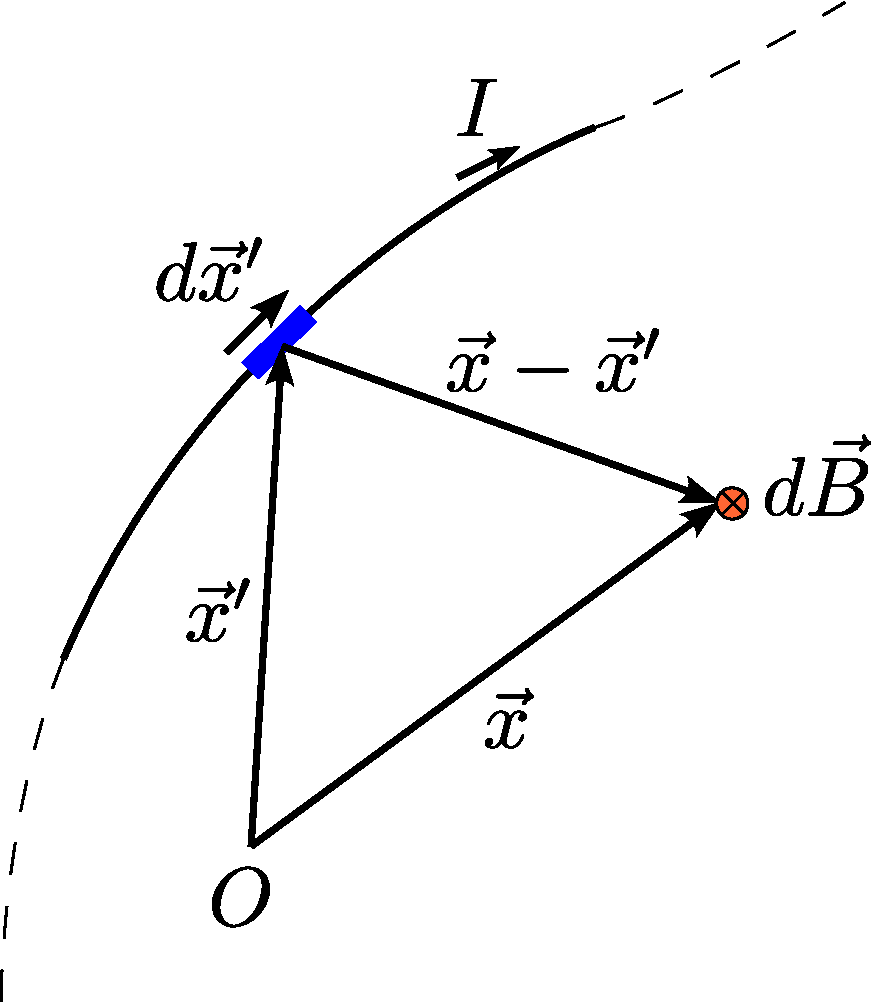
\psfig{file=fig/fig-Biot-Savart-01.pdf,height=6cm,angle=0}}
\label{Esquema para la ley de Biot-Savart.}
\label{fBS1}
\caption{Ley de Biot-Savart.}
\end{figure}
En resumen,
\begin{equation}
dB_i=kI\varepsilon_{ijk}dx'_j\frac{\left(x_k-x'_k\right)}{\left\vert
\vec{x}-\vec{x}'\right\vert^3},
\end{equation}
donde $k$ es una constante, que depende del sistema de unidades usado y que,
en el Sistema Internacional, \textit{se define} como
\begin{equation}
k=\frac{\mu_0}{4\pi}=10^{-7}~\left[  \frac{V\,s}{A\,m}\right],
\end{equation}
y donde $\mu_0$ es llamada la constante de \textbf{permeabilidad magn'etica del vac'io}.

Con esto, escribimos la \textbf{ley de Biot-Savart} como
\begin{equation}
dB_i=\frac{\mu_0}{4\pi}I\,\varepsilon_{ijk}dx'_j\frac{\left(x_k-x'_k\right)}
{\left\vert \vec{x}-\vec{x}'\right\vert ^3}.
\end{equation}
Usando el \textbf{principio de superposici'on} obtenemos una expresi'on para el campo producido por un cable de longitud finita, pero muy delgado:
\begin{equation}
\boxed{B_i(x)=\frac{\mu_0}{4\pi}\int_{\cal C}\varepsilon_{ijk}Idx'_j
\frac{\left(x_k-x'_k\right)}{\left\vert\vec{x}-\vec{x}'\right\vert^3}.}
\label{BS1}
\end{equation}

Podemos generalizar este resultado al caso de una distribuci'on volum'etrica de corriente, descrita por su densidad de corriente. Para esto, consideramos un peque\~no ``tubo de corriente"\, de secci'on transversal $dS$ que sigue las l'ineas de flujo, es decir, tal que el vector normal a la superficie transversal, $\hat{n}$, es paralalo a $\vec{J}$. Entonces, $\vec{J}=J\hat{n}$, $d\vec{x}=d\ell\,\hat{n}$, y adem'as $dV=d\ell\, dS$ (ver figura \ref{fig:tc}), de modo que podemos escribir
\begin{equation}
I\, d\vec{x}=(J dS)(\hat{n}d\ell)=(J\hat{n})(d\ell dS)=\vec{J}\,dV.
\end{equation}
\begin{figure}[!h]
\centerline{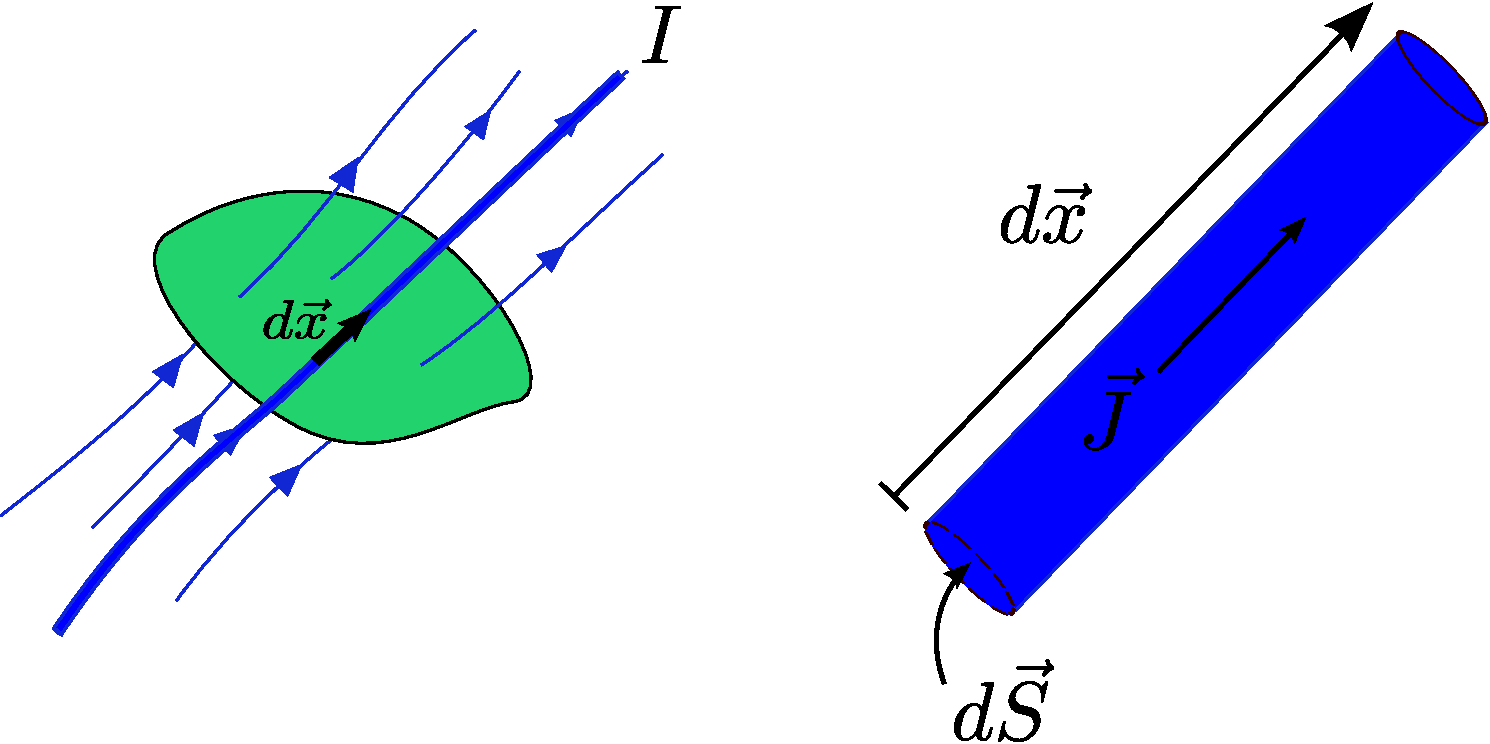
\psfig{file=fig/fig-tubo-de-corriente.pdf,height=4cm,angle=0}}
\caption{Una distribuci'on volum'etrica y los ``tubos de corriente'' asociados.}
\label{fig:tc}
\end{figure}
Con esto podemos encontrar la forma general que usaremos para la ley de Biot-Savart:
\begin{equation}\marginnote{Ley de Biot-Savart}
 \boxed{B_i(x)=\frac{\mu_0}{4\pi}\int_V\varepsilon_{ijk}\,J_j(x')
\frac{\left(x_k-x'_k\right)}{\left\vert\vec{x}-\vec{x}'\right\vert^3}dV'. }
\label{BS2}
\end{equation}
Tambi'en podemos considerar una \textit{distribuci'on superficial de corriente}, es decir una situaci'on donde puede \textit{aproximarse} que la corriente est'a confinada sobre una superficie (de ancho nulo). Para describir esta distribuci'on usamos la \textbf{densidad superficial de corriente}, que denotaremos como $\vec{j}$. Esta densidad superficial es definida tal que
\begin{equation}
\vec{J}\,dV=\vec{j}\,dS,
\end{equation}
donde $dS$ denota el elemento de superficie \textit{sobre} (y no \textit{a trav'es} de) la que fluye la corriente. El campo magn'etico generado por este tipo de distribuciones adopta entonces la forma siguiente:
\begin{equation}
 \boxed{B_i(x)=\frac{\mu_0}{4\pi}\int_S\varepsilon_{ijk}\,j_j(x')
\frac{\left(x_k-x'_k\right)}{\left\vert\vec{x}-\vec{x}'\right\vert^3}dS'. }
\label{BSsup}
\end{equation}
Tal como en el estudio del campo electrost'atico, trabajaremos con la expresi'on volum'etrica \eqref{BS1}, que es m'as general. Si se requiere adaptar las expresiones al caso de corrientes superficiales o lineales pueden entonces usarse las siguientes reglas de conversi'on:
\begin{equation}\label{IdxJdV}
\vec{J}\,dV=\vec{j}\,dS=I\,d\vec{x}.
\end{equation}
Note adem'as que si la corriente es siempre producida por una distribuci'on de cargas movi'endose con velocidad $\vec{v}$ entonces 
\begin{equation}
\vec{J}=\rho\vec{v}, \qquad \vec{j}=\sigma\vec{v}, \qquad I=\lambda v,
\end{equation}
donde $\rho$, $\sigma$ y $\lambda$ son las densidad de carga por unidad de volumen, superficie y longitud, en el caso de distribuciones de corriente volum'etrica, superficial y lineal, respectivamente.

\section{Potencial vectorial}
Consideramos ahora la identidad
\begin{equation}
\frac{x_k-x'_k}{\left\vert
\vec{x}-\vec{x}'\right\vert^3}\equiv -\partial_k\left(
\frac{1}{\left\vert\vec{x}-\vec{x}'\right\vert }\right).
\end{equation}
Reemplaz'andola en (\ref{BS2}) encontramos
\begin{eqnarray}
 B_i(x)&=&-\frac{\mu_0}{4\pi}\int_V\varepsilon_{ijk}\,J_j(x')
\partial_k\left(\frac{1}{\left\vert\vec{x}-\vec{x}'\right\vert }\right)dV'
\label{BS3} \\
&=&-\varepsilon_{ijk}\,\partial_k\left(\frac{\mu_0}{4\pi}\int_VJ_j(x')\frac{1}{
\left\vert\vec{x} -\vec{x}'\right\vert }dV'\right)\\
&=&\varepsilon_{ijk}\,\partial_j\left(\frac{\mu_0}{4\pi}\int_VJ_k(x')\frac{1}{
\left\vert\vec{x} -\vec{x}'\right\vert }dV'\right).
\end{eqnarray}
Por lo tanto, siempre es posible escribir el campo magnetost'atico como el rotor de un campo vectorial,
\begin{equation}\marginnote{Potencial Vectorial}
\boxed{B_i(x)=\varepsilon_{ijk}\,\partial_jA_k(x),}\label{rot-A}
\end{equation}
donde hemos introducido el \textbf{potencial vectorial},
\begin{equation}\marginnote{Pot. Vectorial particular}
\boxed{A_k(x):=\frac{\mu_0}{4\pi}\int_V\frac{J_k(x')}{\left\vert\vec{x}-\vec{x}
'\right\vert }\,dV'.}
\label{defA}
\end{equation}
An'alogamente al caso electrost'atico, el \textit{potencial vectorial no es \'{u}nico}. En el caso magn'etico, sin embargo, la situaci'on es algo menos trivial ya que es posible considerar un nuevo potencial vectorial
\begin{equation}
A'_i:=A_i+\partial_i\Psi(x), \label{gauge01}
\end{equation}
donde $\Psi(x)$ es una \textit{funci'on arbitraria}, y el campo magn'etico
permanecer'a inalterado, ya que $B'_i(x)=\varepsilon_{ijk}\,\partial_jA'_k(x)=B_i(x)$. La transformaci'on (\ref{gauge01}) es llamada una \textbf{transformaci'on de gauge}
del potencial vectorial. Como consecuencia, el potencial vectorial $\vec{A}(x)$
\textit{no es una cantidad medible}, sino m'as bien un campo auxiliar (muy)
'util en muchos c'alculos. En general, a menos que se explicite lo contrario,
cuando hablemos del potencial vectorial magn'etico nos referiremos la elecci'on particular 
dada por (\ref{defA}).


\section{Divergencia del Campo Magn'etico}

Como consecuencia directa de (\ref{rot-A}), vemos que \textit{el campo magnetost'atico
es siempre libre de divergencia}:
\begin{equation}
 \boxed{\vec{\nabla}\cdot\vec{B}=0.} \label{divB}
\end{equation}
Equivalentemente,
\begin{equation}
 \oint_S\vec{B}\cdot d\vec{S}=0,
\end{equation}
es decir, que el \textbf{flujo magn'etico} a trav'es de cualquier superficie cerrada es nulo.

Recordemos que el flujo magn'etico a trav'es de una superficie $S$ es definido
como
\begin{equation}
 \Phi_S:= \int_S\vec{B}\cdot d\vec{S}.
\end{equation}
Usando (\ref{rot-A}) y el teorema de Stokes encontramos que
\begin{equation}\label{PAdx}
 \Phi_S=\oint_{\partial S}\vec{A}\cdot d\vec{x},
\end{equation}
es decir, que el flujo magn'etico a trav'es de una superficie s'olo depende del
valor del potencial vectorial sobre la curva (orientada) $\partial S$ que delimita $S$.
Puede verificarse adem'as que, si bien la expresi'on anterior involucra el
potencial vectorial, \textit{el valor del flujo $\Phi_S$ es independiente de la
elecci'on particular de $\vec{A}$} dentro de la familia de potenciales
vectoriales asociados a un campo $\vec B$ dado. En otras palabras el flujo es
\textbf{invariante} bajo transformaciones de gauge. Note adem'as que, debido a la
relaci'on entre $\Phi_S$ y $\vec{B}$ este 'ultimo vector es tambi'en llamado
\textbf{densidad de flujo magn'etico}. En el sistema internacional de unidades, se define el \textit{Weber}\footnote{En honor a Wilhelm Weber, f'isico alem'an (1804-1891). Ver \url{http://es.wikipedia.org/wiki/Wilhelm_Weber}.} como unidad de flujo magn'etico: $1Wb=1T\cdot 1m^2=1V\cdot 1s$.

\section{Ley de Amp\`ere}

Queremos calcular el rotor de la intensidad de campo magn'etico, es decir, $\varepsilon_{ijk}\partial_jB_k$. Usando (\ref{rot-A})
podemos escribir:
\begin{eqnarray}
 \varepsilon_{ijk}\partial_jB_k&=&\varepsilon_{ijk}\varepsilon_{
klm}\partial_j\partial_lA_m \\
&=&\partial_i(\partial_jA_j) -\partial_j\partial_jA_i. \label{rotB1}
\end{eqnarray}
Para evaluar esta expresi'on usaremos el potencial definido por (\ref{defA})
(el resultado final es independiente de la elecci'on de $\vec{A}$ ya que s'olo
depende de $\vec{B}$). Calculemos primero la divergencia del potencial
vectorial:
\begin{eqnarray}
\partial_iA_i&=&\frac{\mu_0}{4\pi}\int_VJ_i(x')\partial_i\frac{1}{\left\vert\vec
{x} -\vec{x}'\right\vert }\,dV' \\
&=& -\frac{\mu_0}{4\pi}\int_VJ_i(x')\partial'_i\frac{1}{\left\vert\vec{
x } -\vec{x}'\right\vert }\,dV' \\
&=&-\frac{\mu_0}{4\pi}\int_V\left[\partial'_i\left(\frac{J_i(x')}{
\left\vert\vec{x}-\vec{x}'\right\vert}\right)-\frac{
\left(\partial'_iJ_i(x')\right) } { \left\vert\vec{x} -\vec{x}'\right\vert
}\right]\,dV' \\
&=&-\frac{\mu_0}{4\pi}\oint_{\partial V}\frac{J_i(x')}{
\left\vert\vec{x}-\vec{x}'\right\vert}dS'_i+\frac{\mu_0}{4\pi}\int_V\frac{
\left(\partial'_iJ_i(x')\right) } {\left\vert\vec{x}
-\vec{x}'\right\vert}\,dV'  \label{divA} \\
&=&0. \label{divA0}
\end{eqnarray}
El primer t'ermino del lado derecho de (\ref{divA}) se anula cuando cuando $V$
se extiende a todo el espacio, puesto que suponemos que la densidad de corriente
se anula suficientemente r'apido en el infinito (m'as r'apido que $1/r$). Adem'as, el segundo t'ermino es nulo \textit{para corrientes estacionarias}, ver (\ref{divJ0}). Por lo tanto, hemos probado que el potencial (\ref{defA}) tiene divergencia nula en el caso de corrientes
estacionarias confinadas a regiones compactas del espacio.

Debemos ahora calcular el laplaciano (de cada una de las componentes) de
$\vec{A}$. De la definici'on (\ref{defA}) encontramos que
\begin{eqnarray}
 \nabla^2A_i&=&\frac{\mu_0}{4\pi}\int_VJ_i(x')\nabla^2\frac{1}{\left\vert\vec{
x } -\vec{x}'\right\vert }\,dV'\\
&=&\frac{\mu_0}{4\pi}\int_VJ_i(x')\left(-4\pi\delta^{(3)}(\vec{x}-\vec{x}
')\right)\,dV' \\
&=&-\mu_0J_i(x). \label{lapAj}
\end{eqnarray}
Reemplazando (\ref{divA0}) y (\ref{lapAj}) en (\ref{rotB1}) encontramos la
\textbf{ley de Amp\`ere}\footnote{\href{http://es.wikipedia.org/wiki/Andr\%C3\%A9-Marie_Amp\%C3\%A8re}{Andr'e-Marie Amp\`ere} (1775-1836): matem'atico y f'isico franc'es.}:
\begin{equation}
\boxed{\varepsilon_{ijk}\partial_jB_k=\mu_0J_i,}
\end{equation}
o, en notaci'on vectorial,
\begin{equation}\marginnote{Ley Amp\`ere (diferencial)}
 \boxed{\vec\nabla\times\vec{B}=\mu_0\vec{J}.}\label{ley-Ampere}
\end{equation}
La versi'on integral de la ley de Amp\`ere (obtenida integrando
(\ref{ley-Ampere}) en una superficie $S$ con borde $\partial S$, y usando el
teorema de Stokes) es
\begin{equation}\marginnote{Ley Amp\`ere (integral)}
 \boxed{\oint_{\partial S}\vec{B}\cdot d\vec{x}=\mu_0 I_S,}
\end{equation}
donde $I_S=\int_S\vec{J}\cdot d\vec{S}$ es la corriente neta que fluye por $S$.

\subsection{Ejemplo: Campo magn'etico producido por una l'inea infinita de
corriente}
\begin{figure}[!h]
\centerline{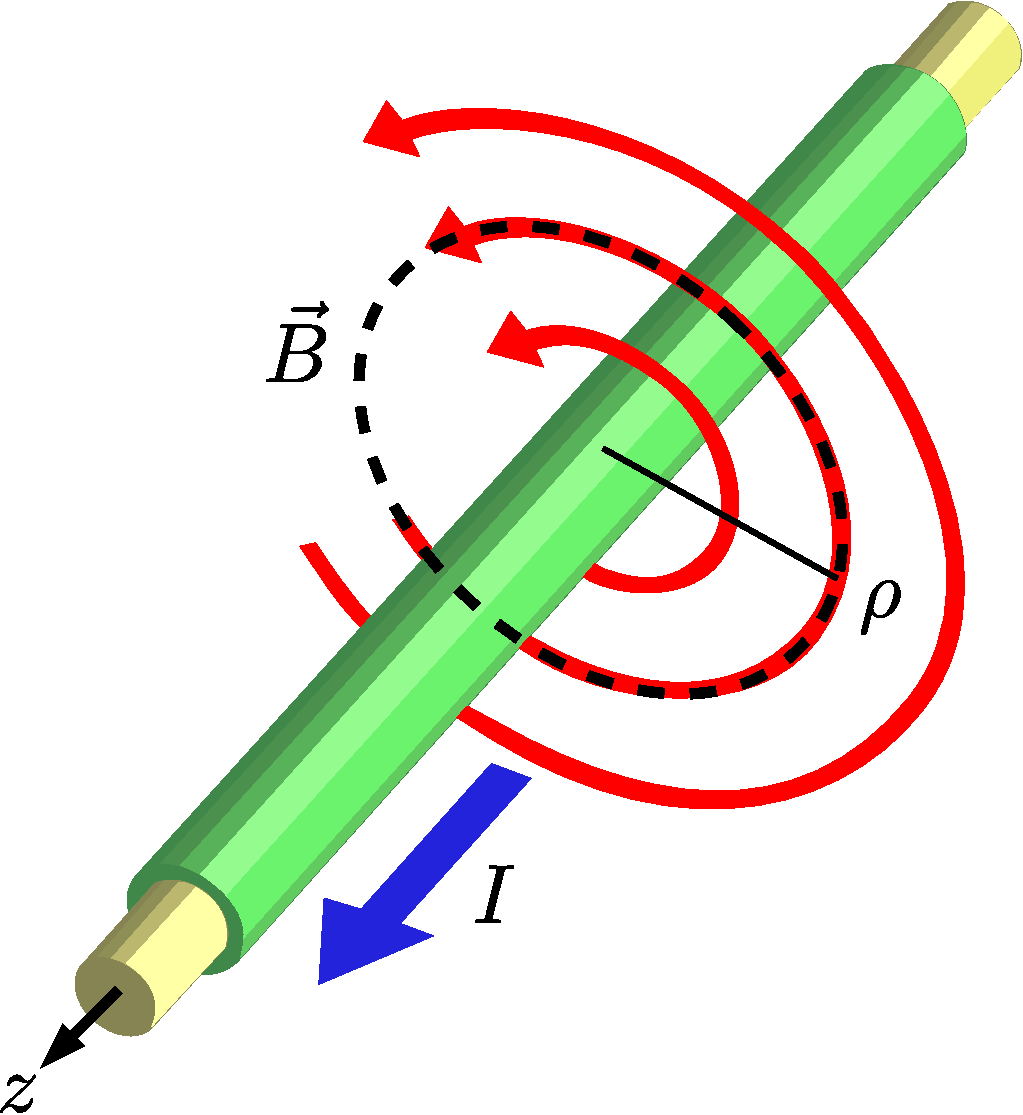
\psfig{file=fig/fig-B-conductor-recto-01.pdf,height=5cm,angle=0}}
\caption{Campo magn'etico producido por un conductor recto. Figura original  \href{http://en.wikipedia.org/wiki/File:Electromagnetism.svg}{aqu\'i}.}
\label{cmcr}
\end{figure}
Aplicando la ley de Amp\`ere a la circunsferencia de radio $\rho$ indicada en la figura
(\ref{cmcr}) encontramos que
\begin{equation}
 \oint_{\cal C}\vec{B}\cdot d\vec{x}=(2\pi \rho)B=\mu_0 I,
\end{equation}
de modo que
\begin{equation}
\vec{B}(\rho)=\frac{\mu_0I}{2\pi}\frac{\hat{\varphi}}{\rho}.
\end{equation}
Un potencial vectorial posible para describir este campo es
\begin{equation}
 \vec{A}_1(\rho)=-\frac{\mu_0I}{2\pi}\ln\frac{\rho}{\rho_0} \hat{z}.
\end{equation}
Sin embargo, otro potencial posible es
\begin{equation}
 \vec{A}_2(z)=\frac{\mu_0I}{2\pi}\frac{z}{\rho} \hat{\rho}.
\end{equation}


\section{Potencial escalar magn'etico}\label{secpem}
En regiones en las que no existen corrientes, $\vec{J}=\vec{0}$, el
rotor del campo magn'etico es nulo, $\vec{\nabla}\times\vec{B}=\vec{0}$. En
este caso es \textit{posible escribir $\vec{B}$ como el gradiente de un campo escalar},
\begin{equation}\marginnote{Potencial Escalar Magn'etico}
 \vec{B}=-\mu_0\vec\nabla\phi^*, \label{Bgradphi}
\end{equation}
donde $\phi^*$ es llamado \textbf{potencial escalar magn'etico}. Ya que adem'as
el campo magn'etico es (siempre) libre de divergencias, tenemos que
\begin{equation}
 \boxed{\nabla^2\phi^*=0,}
\end{equation}
\textit{en regiones sin corrientes}.

Esta propiedad permite en muchos casos aplicar m'etodos similares a aquellos de
la electrost'atica, para determinar el potencial (magn'etico, en este caso)
como soluci'on de la ecuaci'on de Laplace en regiones libres de corrientes,
imponiendo las condiciones de contorno adecuadas para el campo magn'etico.

\section{Expansi'on multipolar magn'etica}\label{sec:emm}
\begin{figure}[!h]
\centerline{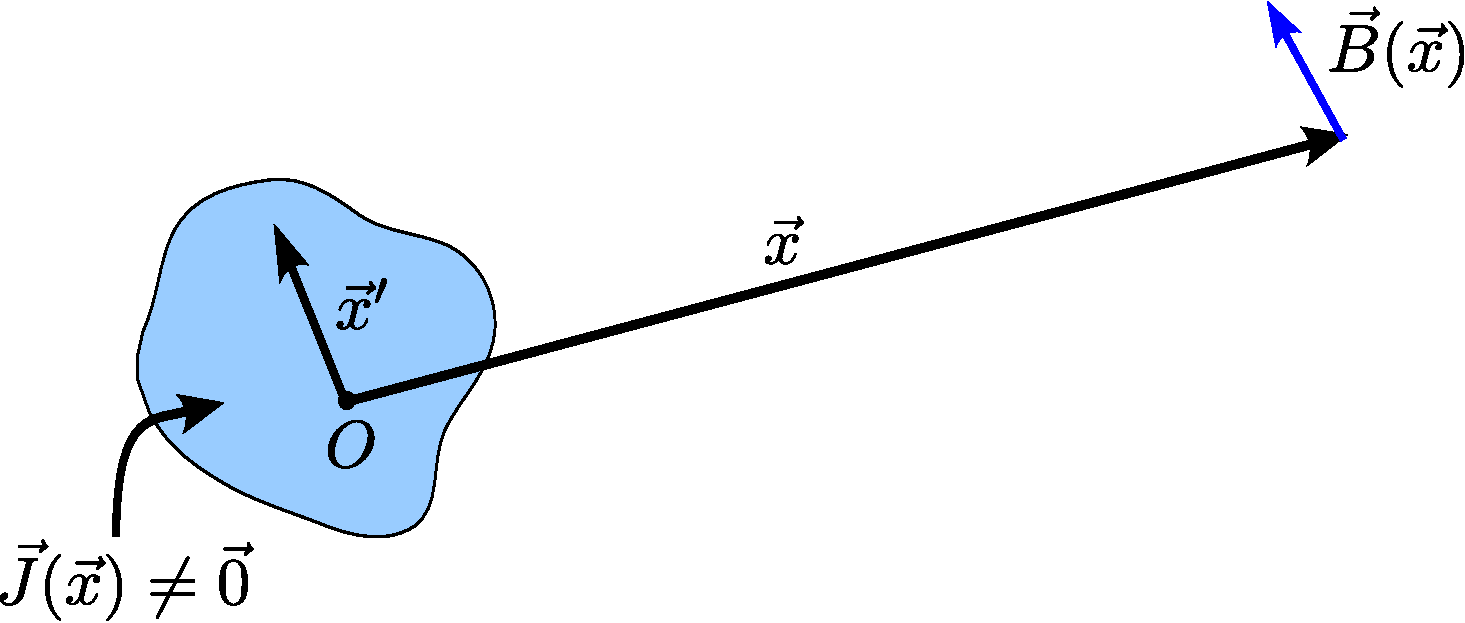
\psfig{file=fig/fig-expansion-multipolar-magnetica-01.pdf,height=4cm,
angle=0 } }
\caption{Esquema de la expansi'on multipolar magn'etica.}
\label{MM1}
\end{figure}
An'alogamente al caso electrost'atico, deseamos calcular el campo
magn'etico $\vec{B}$ lejos de una distribuci'on  de corrientes, descritas por una densidad de corriente $\vec{J}$, localizada en una regi'on peque\~na comparada con la distancia a la cual se calcular'a el campo.

Situando el origen en un punto representativo de la distribuci'on de
corrientes, tendremos que para distancias grandes comparadas con el
tama\~no de la distribuci'on se satisface $\left\vert\vec{x}\right\vert \gg\left\vert
\vec{x}'\right\vert $,\ ver figura \ref{MM1}. Con esto, podemos usar la
expansi'on (\ref{exp1or}) y reescribir la expresi'on (\ref{defA}) como una
expansi'on multipolar magn'etica:
\begin{equation}
 A_i(x)=\frac{\mu_0}{4\pi}\sum_{n=0}^\infty \frac{(-1)^n}{n!}M_{i_1\cdots
i_ni}\partial_{i_1}\cdots \partial_{i_n}\frac{1}{r},
\end{equation}
donde hemos definidos los \textbf{momentos multipolares magn'eticos} como
\begin{equation}
\boxed{ M_{i_1\cdots i_ni}:=\int_V x_{i_1}\cdots x_{i_n}\,J_i(x)\,dV.}
\end{equation}
Note que, debido al caracter vectorial de la densidad de corriente, el momento
multipolar magn'etico de orden $n$ es un tensor de orden $n+1$.

En la pr'actica es com'un usar s'olo los primeros t'erminos de la expansi'on
multipolar magn'etica. Adem'as, el t'ermino monopolar magn'etico es siempre
identicamente nulo \textit{para corrientes estacionarias}, ya que
\begin{equation}
 M_i=\int_V J_i(x)\,dV=0. \label{mmm0}
\end{equation}
Para probar esto, considere la siguiente integral $\oint_{\partial V}x_i
J_j\,dS_j$. Usando el teorema de Gauss podemos escribir
\begin{equation}
 \oint_{\partial V}x_i
J_j\,dS_j=\int_V\partial_j(x_iJ_j)\,dV=\int_V\left[
(\partial_jx_i)J_j+x_i(\partial_jJ_j)\right]\,dV=\int_V\left[
\delta_{ij}J_j+0\right]\,dV
\end{equation}
En la 'ultima igualdad usamos el hecho que para corrientes estacionarias la
divergencia del vector densidad de corriente es nula, ver \eqref{divJ0}. Con esto, encontramos la
identidad
\begin{equation}
  \int_VJ_i\,dV\equiv \oint_{\partial V}x_iJ_j\,dS_j.
\end{equation}
Esta identidad es v'alida para cualquier volumen $V$. Entonces para probar lo
requerido basta considerar un volumen que \textit{contiene totalmente}
la distribuci'on de corrientes, de modo que $\vec{J}=\vec{0}$ en la superficie
$\partial V$.

Este resultado general (para corrientes estacionarias) tiene como consecuencia
que \textit{la expansi'on multipolar magn'etica comienza con el t'ermino
dipolar} ($n=1$).

El momento multipolar de orden 1 es dado por
\begin{equation}
 M_{ij}=\int_V x_i\,J_j(x)\,dV.
\end{equation}

Es posible probar que este tensor es \textit{antisim'etrico},
$M_{ij}=-M_{ji}$, \textit{para distribuciones de corrientes estacionarias}. Para esto,
basta analizar la integral $\oint_{\partial V}x_i x_j J_k\,dS_k$ de forma
an'aloga a lo discutido anteriormente, es decir, aplicando el teorema de Gauss y la
condici'on de divergencia nula de la densidad de corriente. Ya que $M_{ij}$ es
antisim'etrico, \textit{la informaci'on que este tensor contiene puede ser
equivalentemente descrita en t'erminos de un (pseudo-) vector} $\vec{\mu}$,
llamado \textbf{momento (dipolar) magn'etico}, y definido por
\begin{equation}
 \mu_i:=\frac{1}{2}\varepsilon_{ijk}M_{jk}, \qquad
M_{ij}=\varepsilon_{ijk}\mu_k, \label{vmdm}
\end{equation}
es decir,
\begin{equation}
 \boxed{\mu_i=\frac{1}{2}\varepsilon_{ijk}\int_V x_j J_k(x)\, dV,}
\end{equation}
o, en notaci'on vectorial, 
\begin{equation}
 \boxed{\vec{\mu}=\frac{1}{2}\int_V \vec{x}\times\vec{J}(x)\,dV,}
\end{equation}
Con esto, el t'ermino dipolar de la expansi'on multipolar magn'etica para el
potencial vectorial \eqref{defA} es
\begin{eqnarray}
 A_i^{(1)}(x)&=&-\frac{\mu_0}{4\pi}M_{ji}\partial_j\frac{1}{r} \\
&=&-\frac{\mu_0}{4\pi}\left(\varepsilon_{jil}\mu_l\right)\left(-\frac{x_j}{
r^3}\right) \\
&=&\frac{\mu_0}{4\pi}\varepsilon_{ijk}\frac{\mu_jx_k}{r^3},
\end{eqnarray}
es decir,
\begin{equation}
 \boxed{\vec{A}^{(1)}(x)=\frac{\mu_0}{4\pi}\frac{\vec{\mu}\times\vec{x}}{r^3}.}
\label{Adip}
\end{equation}
M'as importante que el potencial, que sabemos no es 'unico, es el campo
magn'etico. La contribuci'on dipolar al campo generado por una distribuci'on
compacta de corriente es entonces dado por
\begin{eqnarray}
B_i^{(1)}(x)&=&\varepsilon_{ijk}\partial_jA_k^{(1)}(x)\\
&=&\varepsilon_{ijk}\partial_j\left(\frac{\mu_0}{4\pi}\varepsilon_{klm}\frac{
\mu_lx_m}{r^3}\right) \\
&=&\frac{\mu_0}{4\pi}\varepsilon_{ijk}\varepsilon_{klm}\mu_l\partial_j\left(
\frac{x_m}{r^3}\right) \\
&=&\frac{\mu_0}{4\pi}\left(\delta_{il}\delta_{jm}-\delta_{jl}\delta_{im}\right)
\mu_l\left(\frac{\delta_{jm}}{r^3}-3\frac{x_mx_j}{r^5}\right) \\
&=&\frac{\mu_0}{4\pi}\left[3\frac{x_i(x_j\mu_j)}{r^5}-\frac{\mu_i}{r^3}
\right] ,
\end{eqnarray}
o, en notaci'on vectorial
\begin{equation}
\boxed{\vec{B}^{(1)}=\frac{\mu_0}{4\pi}\left[\frac{3\hat{r}(\vec{\mu}
\cdot\hat{r}) -\vec{\mu}}{r^3}\right] , \qquad \hat{r}:=\frac{\vec{x}}{r}.}
\end{equation}
\begin{figure}[!h]
\centerline{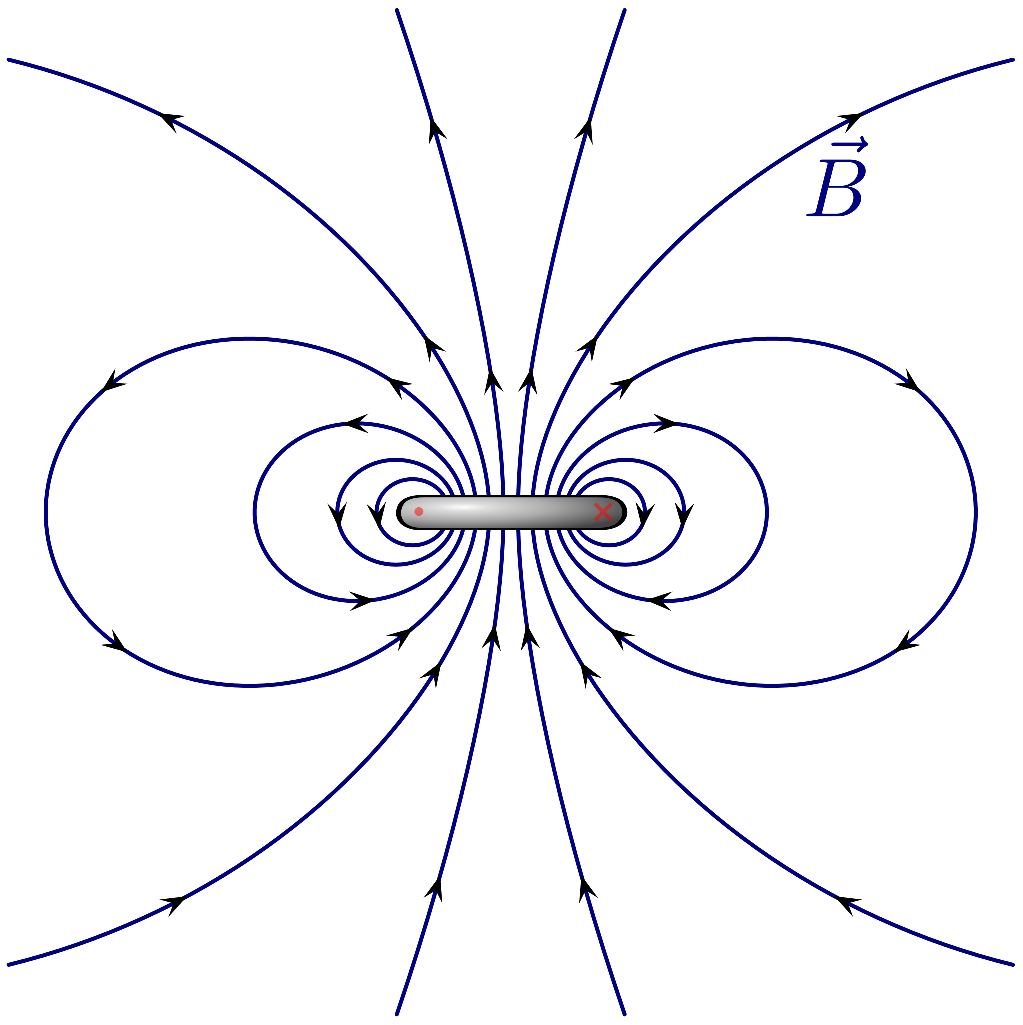
\psfig{file=fig/fig-campo-magnetico-espira.pdf,height=5cm,angle=0}\hspace{2cm}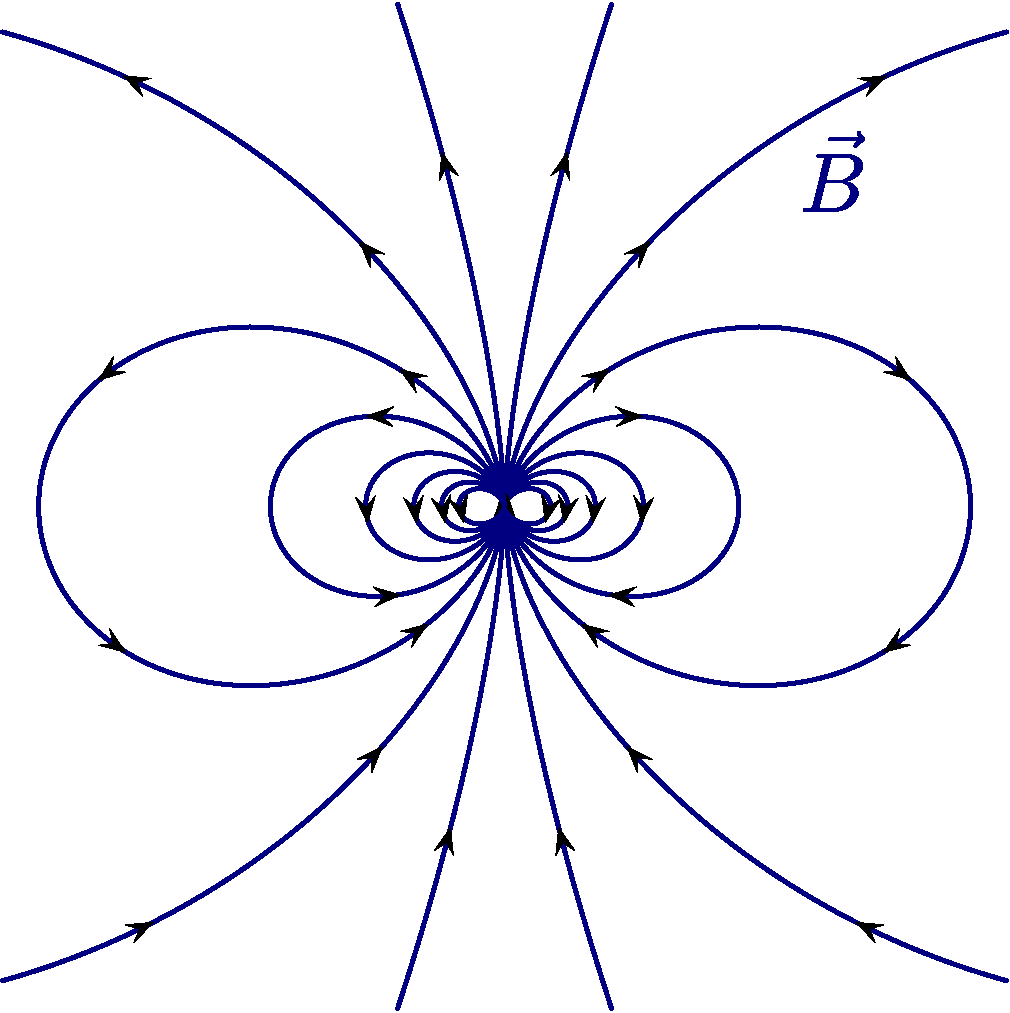
\psfig{file=fig/fig-campo-dipolo-magnetico.pdf,height=5cm,angle=0}}
\caption{a) Campo magn'etico de una espira, b) campo magn'etico de un dipolo ideal. Adaptadas a partir de \href{http://commons.wikimedia.org/wiki/File:VFPt_dipole_point.svg}{esta} y \href{http://commons.wikimedia.org/wiki/File:VFPt_dipole_magnetic3.svg}{esta} figuras originales.}
\label{fig:dipmag}
\end{figure}

\subsection{Momento dipolar de una espira plana}
\begin{figure}[!h]
\centerline{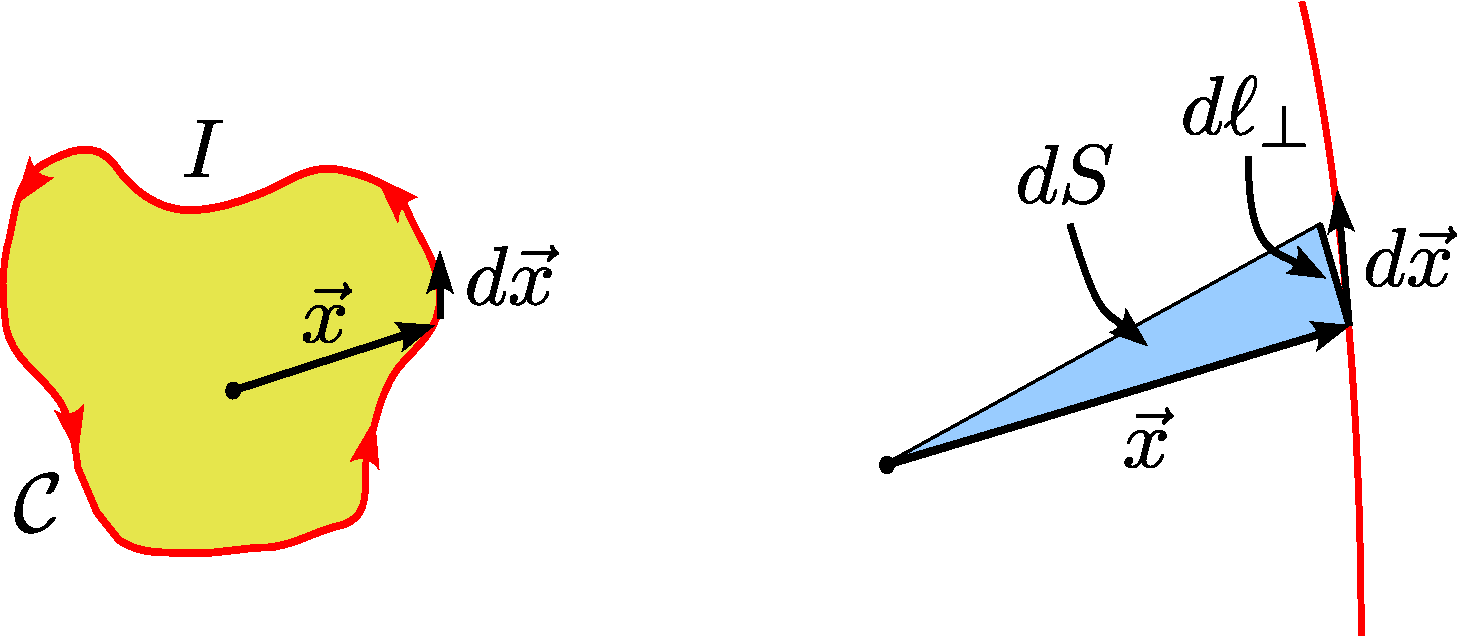
\psfig{file=fig/fig-espira-plana-01.pdf,height=4cm,angle=0}}
\caption{Espira plana y elemento de 'area.}
\label{fep01}
\end{figure}
En el caso de que la distribuci'on de corriente se concentre en conductores que
describen una curva $\cal C$ (sobre un plano) y transportan corriente $I$, el momento magn'etico
es dado por
\begin{equation}\label{muintC}
 \vec{\mu}=\frac{I}{2}\oint_{\cal C} \vec{x}\times d\vec{x}.
\end{equation}
En el caso de un \textit{espira plana}, pero de forma arbitraria, tenemos que
(situando el origen en un punto del mismo plano), $\vec{x}\times
d\vec{x}/2=rd\ell_\bot\hat{n}/2=dS\,\hat{n}$, donde $\hat{n}$ es el
vector normal a la espira cuya con direcci'on dada por la regla de la mano
derecha aplicada a la curva orientada de acuerdo al sentido de circulaci'on de
la corriente\footnote{Equivalentemente, puede obtener este resultado a partir de \eqref{muintC} usando el teorema de Stokes.}. Con esto obtenemos que el momento magn'etico de una espira plana
de 'area $A$ es siempre de la forma
\begin{equation}\marginnote{Momento magn'etico espira plana}
 \boxed{\vec{\mu}=IA\,\hat{n}.}
\end{equation}

\subsection{Relaci'on entre momento magn'etico y momento angular}
En algunos sistemas se tiene que la densidad de carga el'ectrica (en cada
punto) es proporcional a la densidad de masa, de modo que
\begin{equation}
 \rho(x)=\frac{Q}{M} \rho_{\rm m}(x).
\end{equation}
donde $Q$ es la carga total y $M$ la masa total del sistema. Esto ocurre, en
general, en sistemas constituidos por \textit{un s'olo tipo de part'iculas},
masivas y cargadas. En este caso, si cada elemento del sistema se mueve
con velocidad $\vec{v}(x)$, entonces
\begin{equation}
\vec{J}=\rho(x)\vec{v}(x)=\frac{Q}{M} \rho_{\rm m}(x)\vec{v}(x)
\end{equation}
y entonces el momento magn'etico puede escribirse como
\begin{equation}
 \vec{\mu}=\frac{1}{2}\int_V \vec{x}\times\vec{J}\,dV=\frac{Q}{2M}\int_V
\vec{x}\times\rho_{\rm m}(x)\vec{v}(x)\,dV=\frac{Q}{2M}\int_V
\vec{x}\times d\vec{p},
\end{equation}
donde $d\vec{p}:=\rho_{\rm m}(x)\vec{v}(x)\,dV$ denota el \textbf{momentum lineal} de la masa en el elemento de volumen $dV$. De esta forma $d\vec{L}:=\vec{x}\times d\vec{p}$ es el \textbf{momento angular} del peque\~no elemento de masa (respecto al origen elegido) y, finalmente,
\begin{equation}
 \boxed{\vec{\mu}=\frac{Q}{2M}\vec{L}.}
\end{equation}

\section{Fuerza y torque sobre una distribuci'on compacta de corriente}
Consideramos ahora el caso en que una peque\~na distribuci'on de corriente
se ubica en una regi'on donde existe un campo magn'etico \textit{externo}
$\vec{B}(x)$.

La fuerza total que la distribuci'on de corrientes experimenta, debido al campo
externo (es decir, sin tomar en cuenta la autointeracci'on de la distribuci'on),
es dada por (\ref{fm1}). Para expresar esta fuerza en t'erminos de los momentos multipolares magn'eticos de la distribuci'on, situamos nuevamente el
origen de coordenadas en un punto representativo de la distribuci'on y expandimos la
intensidad de campo magn'etico en puntos dentro de 'esta en una serie
de potencias de las componentes del $\vec{x}'$:
\begin{align}
 B_i(\vec{x}+\vec{x}') &= \sum_{n=0}^\infty \frac{1}{n!}x'_{i_1}\cdots x'_{i_n}(\partial_{i_1}\cdots\partial_{i_n}B_i)(x) \label{expB} \\
 &= B_i(x)+x'_j(\partial_jB_i)(x) +
\frac{1}{2}x'_jx'_k(\partial_j\partial_kB_i)(x)+\cdots .
\end{align}
Reemplazando esto en (\ref{fm1}), y tomando en cuenta que la integral sobre la regi'on con corrientes es sobre la variable $\vec{x}'$, encontramos
\begin{align}
F^{\rm m}_i &=  \varepsilon_{ijk}\sum_{n=0}^\infty\frac{1}{n!}M_{i_1\cdots i_nj}(\partial_{i_1}\cdots\partial_{i_n}B_k)(x)\\
&= \varepsilon_{ijk}\left[M_jB_k(x)+M_{lj}(\partial_lB_k)(x)+\frac{1}{2}M_{lnj}(\partial_l\partial_nB_k)(x) +\cdots\right].
\end{align}
Usando (\ref{mmm0}) y (\ref{vmdm}) obtenemos
\begin{eqnarray}
F^{\rm m}_i
&=&\varepsilon_{ijk}\varepsilon_{ljm}\,\mu_m (\partial_lB_k)(x)+\cdots \\
&=& \mu_j(\partial_iB_j)(x)-\mu_i(\partial_jB_j)(x)+\cdots .
\end{eqnarray}
Finalmente, usando la ecuaci'on de campo (\ref{divB}) llegamos a
\begin{equation}
 \boxed{F^{\rm m}_i=\mu_j(\partial_iB_j)(x)+\cdots .}
\end{equation}
En otras palabras, la primera contribuci'on en la expansi'on multipolar a la
fuerza neta sobre una distribuci'on arbitraria es dada por el t'ermino dipolar,
con
\begin{equation}
 \boxed{F_i^{\rm m,(1)}=-\partial_i U_{\rm m}, }
\end{equation}
donde hemos introducido la \textbf{energ'ia de interacci'on entre un dipolo magn'etico
y un campo externo}
\begin{equation}
 \boxed{U_{\rm m}(x)=-\vec{\mu}\cdot\vec{B}(x).} \label{Umagdip}
\end{equation}

Similarmente, el torque neto sobre la espira (con respecto al punto de referencia $O$)  puede calcularse a partir de
\begin{equation}
 \tau_i=\varepsilon_{ijk}\int_V x'_j f^{\rm m}_k(x') dV',
\end{equation}
donde $f^{\rm m}_k$ son las componentes de la densidad de fuerza magn'etica,
definida en (\ref{dfm}). Por lo tanto, usando nuevamente la expansi'on
(\ref{expB}) podemos escribir,
\begin{eqnarray}
  \tau_i&=&\varepsilon_{ijk}\varepsilon_{kln}\int_V x'_j J_l(x')B_n(x')\, dV' \\
&=&\varepsilon_{ijk}\varepsilon_{kln}\int_V x'_j
J_l(x')\left[B_n(x)+x'_p(\partial_pB_n)_(x) +\cdots\right] dV \\
&=&\varepsilon_{ijk}\varepsilon_{kln}\left[M_{jl}B_n(x)+M_{jpl}(\partial_pB_n)(x)
+\cdots\right] \\
&=&\varepsilon_{ijk}\varepsilon_{kln}\varepsilon_{jlp}\,\mu_pB_n(x)+\cdots\\
&=&\varepsilon_{ijk}\,\mu_jB_k(x)+\cdots 
\end{eqnarray}
o, en notaci'on vectorial
\begin{equation}
 \boxed{\vec{\tau}=\vec{\mu}\times\vec{B}+\cdots .} \label{torqueB}
\end{equation}
Puede verificarse usando (\ref{Umagdip}) y (\ref{torqueB}) que un dipolo
magn'etico (o, en primera aproximaci'on, toda distribuci'on compacta de
corriente) situado en un campo (homog'eneo) externo experimentar'a un torque
que tender'a a \textit{alinear} el momento magn'etico de la distribuci'on con el
del campo externo. La posici'on de equilibrio corresponde al caso en que
$\vec{\mu}$ es paralelo a $\vec{B}$, que es adem'as un equilibrio estable ya
que la energ'ia de interacci'on es m'inima. M'as generalmente, el momento
magn'etico puede realizar un \textbf{movimiento de precesi'on} en torno al campo
magn'etico.

%\subsection{Ejemplo: Precesi'on de Larmor}

\section{Campos magn'eticos en la materia}
An'alogamente al caso electrost'atico, en el que un medio se polariza en
presencia de un campo externo, 'este puede adem'as \textit{magnetizarse}. Esto
significa que en cada peque\~no elemento de volumen (macrosc'opico) puede existir un momento magn'etico no nulo. Este momento magn'etico puede ser producto de
los peque\~nos ``loops''\, de corrientes inducidas por el campo aplicado sobre los
electrones at'omicos. Este tipo de dipolos se inducen en \textit{direcci'on contraria}
al campo aplicado, por lo que tienden a \textit{reducir} el valor de la inducci'on
magn'etica al interior del material. Los materiales \textbf{diamagn'eticos} son aquellos en que este tipo de magnetizaci'on es dominante. El hecho que las
part'iculas subat'omicas, y en particular los electrones, posean \textit{momentos
magn'eticos intr'insecos} (permanentes), hace posible que un material presente
magnetizaci'on no nula, de origen distinto a la generada por las corrientes
inducidas. En general, un campo magn'etico aplicado tender'a a alinear, en
mayor o menor medida, los momentos magn'eticos permanentes del material con el campo aplicado, pudiendo compensar y revertir la magnetizaci'on debida a las corrientes
inducidas. Los materiales paramagn'eticos presentan momentos magn'eticos
netos en la misma direcci'on del campo aplicado. En los ferromagnetos, por
otro lado, la alineaci'on de los momentos magn'eticos permanentes es tal que el
momento magn'etico total es no nulo en ausencia de un campo aplicado, y puede asumir valores varios ordenes de magnitud mayor que el caso de los paramagnetos.

\subsection{Magnetizaci'on}
En resumen, consideraremos que en el interior de un medio, existen momentos
magn'eticos distribuidos en su interior. Modelaremos esta distribuci'on
definiendo el \textbf{(pseudo-)vector de magnetizaci'on} como la densidad de momento
magn'etico, es decir, como el momento magn'etico por unidad de volumen en una
peque\~na regi'on ($\Delta V\to 0$, desde el punto de vista macrosc'opico) del
material:
\begin{equation}\marginnote{Definici'on Magnetizaci'on}
\vec{M}(x):= \lim_{\Delta V\to 0} \frac{\Delta \vec{\mu}}{\Delta V}.
\end{equation}
Como consecuencia, la magnetizaci'on tiene unidades de corriente por unidad de
longitud: $[\vec{M}]={[\vec{\mu}]}/{L^3}={IL^2}/{L^3}={I}/{L}$.
Con esta definici'on, tenemos que el momento magn'etico $d\vec{\mu}(x)$
contenido en un elemento de volumen (macrosc'opico) $dV$ centrado en un punto con  posici'on
$\vec{x}$ es
\begin{equation}
d\vec{\mu}(x)=\vec{M}(x)\,dV.
\end{equation}
Entonces, a partir de (\ref{Adip}) podemos calcular al campo (potencial
vectorial) producido por la distribuci'on de momentos dipolares como la
superposici'on del campo correspondiente al momento dipolar magn'etico contenido en cada
elemento de volumen:
\begin{eqnarray}
 A_i^{\rm M}(x)&=&\frac{\mu_0}{4\pi}\varepsilon_{ijk}\int_V
\frac{d\mu_j(x')(x_k-x'_k)}{ \left\vert\vec{x} -\vec{x}'\right\vert^3} \\
&=& \frac{\mu_0}{4\pi}\varepsilon_{ijk}\int_V \frac{M_j(x')(x_k-x'_k)}{
\left\vert\vec{x} -\vec{x}'\right\vert^3}dV'.
\end{eqnarray}
Usando la identidad (\ref{id01}) podemos escribir este potencial vectorial
producido por la magnetizaci'on del material como:
\begin{eqnarray}
  A_i^{\rm M}(x)&=& \frac{\mu_0}{4\pi}\varepsilon_{ijk}\int_V
M_j(x')\partial'_k\frac{1}{\left\vert\vec{x} -\vec{x}'\right\vert}dV'
\label{AM1}\\
&=& \frac{\mu_0}{4\pi}\varepsilon_{ijk}\int_V\left[\partial'_k\left(
\frac{M_j(x')}{\left\vert\vec{x}
-\vec{x}'\right\vert}\right)-\frac{(\partial'_kM_j(x'))}{\left\vert\vec{x}
-\vec{x}'\right\vert}\right]dV' \\
&=&\frac{\mu_0}{4\pi}\oint_{\partial
V}\frac{\varepsilon_{ijk}M_j(x')}{\left\vert\vec{x}
-\vec{x}'\right\vert}dS'_k+\frac{\mu_0}{4\pi}\int_V\frac{(\varepsilon_{ijk}
\partial'_jM_k(x'))}{ \left\vert\vec{x}-\vec{x}'\right\vert}dV' \\
&=&\frac{\mu_0}{4\pi}\oint_{\partial
V}\frac{(\varepsilon_{ijk}M_j(x')\hat{n}_k)}{\left\vert\vec{x}
-\vec{x}'\right\vert}dS'+\frac{\mu_0}{4\pi}\int_V\frac{(\varepsilon_{ijk}
\partial'_jM_k(x'))}{ \left\vert\vec{x}-\vec{x}'\right\vert}dV'  \\
&=&\frac{\mu_0}{4\pi}\oint_{\partial
V}\frac{j^{\rm M,S}_i(x')}{\left\vert\vec{x}
-\vec{x}'\right\vert}dS'+\frac{\mu_0}{4\pi}\int_V\frac{J^{\rm M}_i(x')}{
\left\vert\vec{x}-\vec{x}'\right\vert}dV'.
\end{eqnarray}
En resumen
\begin{equation}
 \boxed{\vec{A}^{\rm M}(x)=\frac{\mu_0}{4\pi}\int_V\frac{\vec{J}^{\rm M}(x')}{
\left\vert\vec{x}-\vec{x}'\right\vert}dV'+\frac{\mu_0}{4\pi}\oint_{\partial
V}\frac{\vec{j}^{\rm M}(x')}{\left\vert\vec{x}-\vec{x}'\right\vert}dS',}
\label{AM01}
\end{equation}
donde hemos definido la \textbf{densidad de corriente de magnetizaci'on}
$\vec{J}^{\rm M}$ y la \textbf{densidad de corriente superficial de
magnetizaci'on} $\vec{j}^{\rm M}$ por
\begin{equation}\marginnote{corrientes de magnetizaci'on}
\boxed{\vec{J}^{\rm M}(x):=\vec\nabla\times\vec{M}(x), \qquad \vec{j}^{\rm
M}(x):=\vec{M}(x)\times\hat{n}(x).}
\end{equation}
Estas definiciones de densidades de corriente, que pueden ser reales o
ficticias dependiendo del origen de la magnetizaci'on $\vec{M}$, son de utilidad
puesto que, de acuerdo a (\ref{AM01}), el campo producido por la magnetizaci'on
es \textit{equivalente} al campo producido (a trav'es de la ley de Biot-Savart)
por las corrientes descritas por $\vec{J}^{\rm M}$ en el interior del material y
por $\vec{j}^{\rm M}$ en su superficie.

\begin{figure}[!h]
\centerline{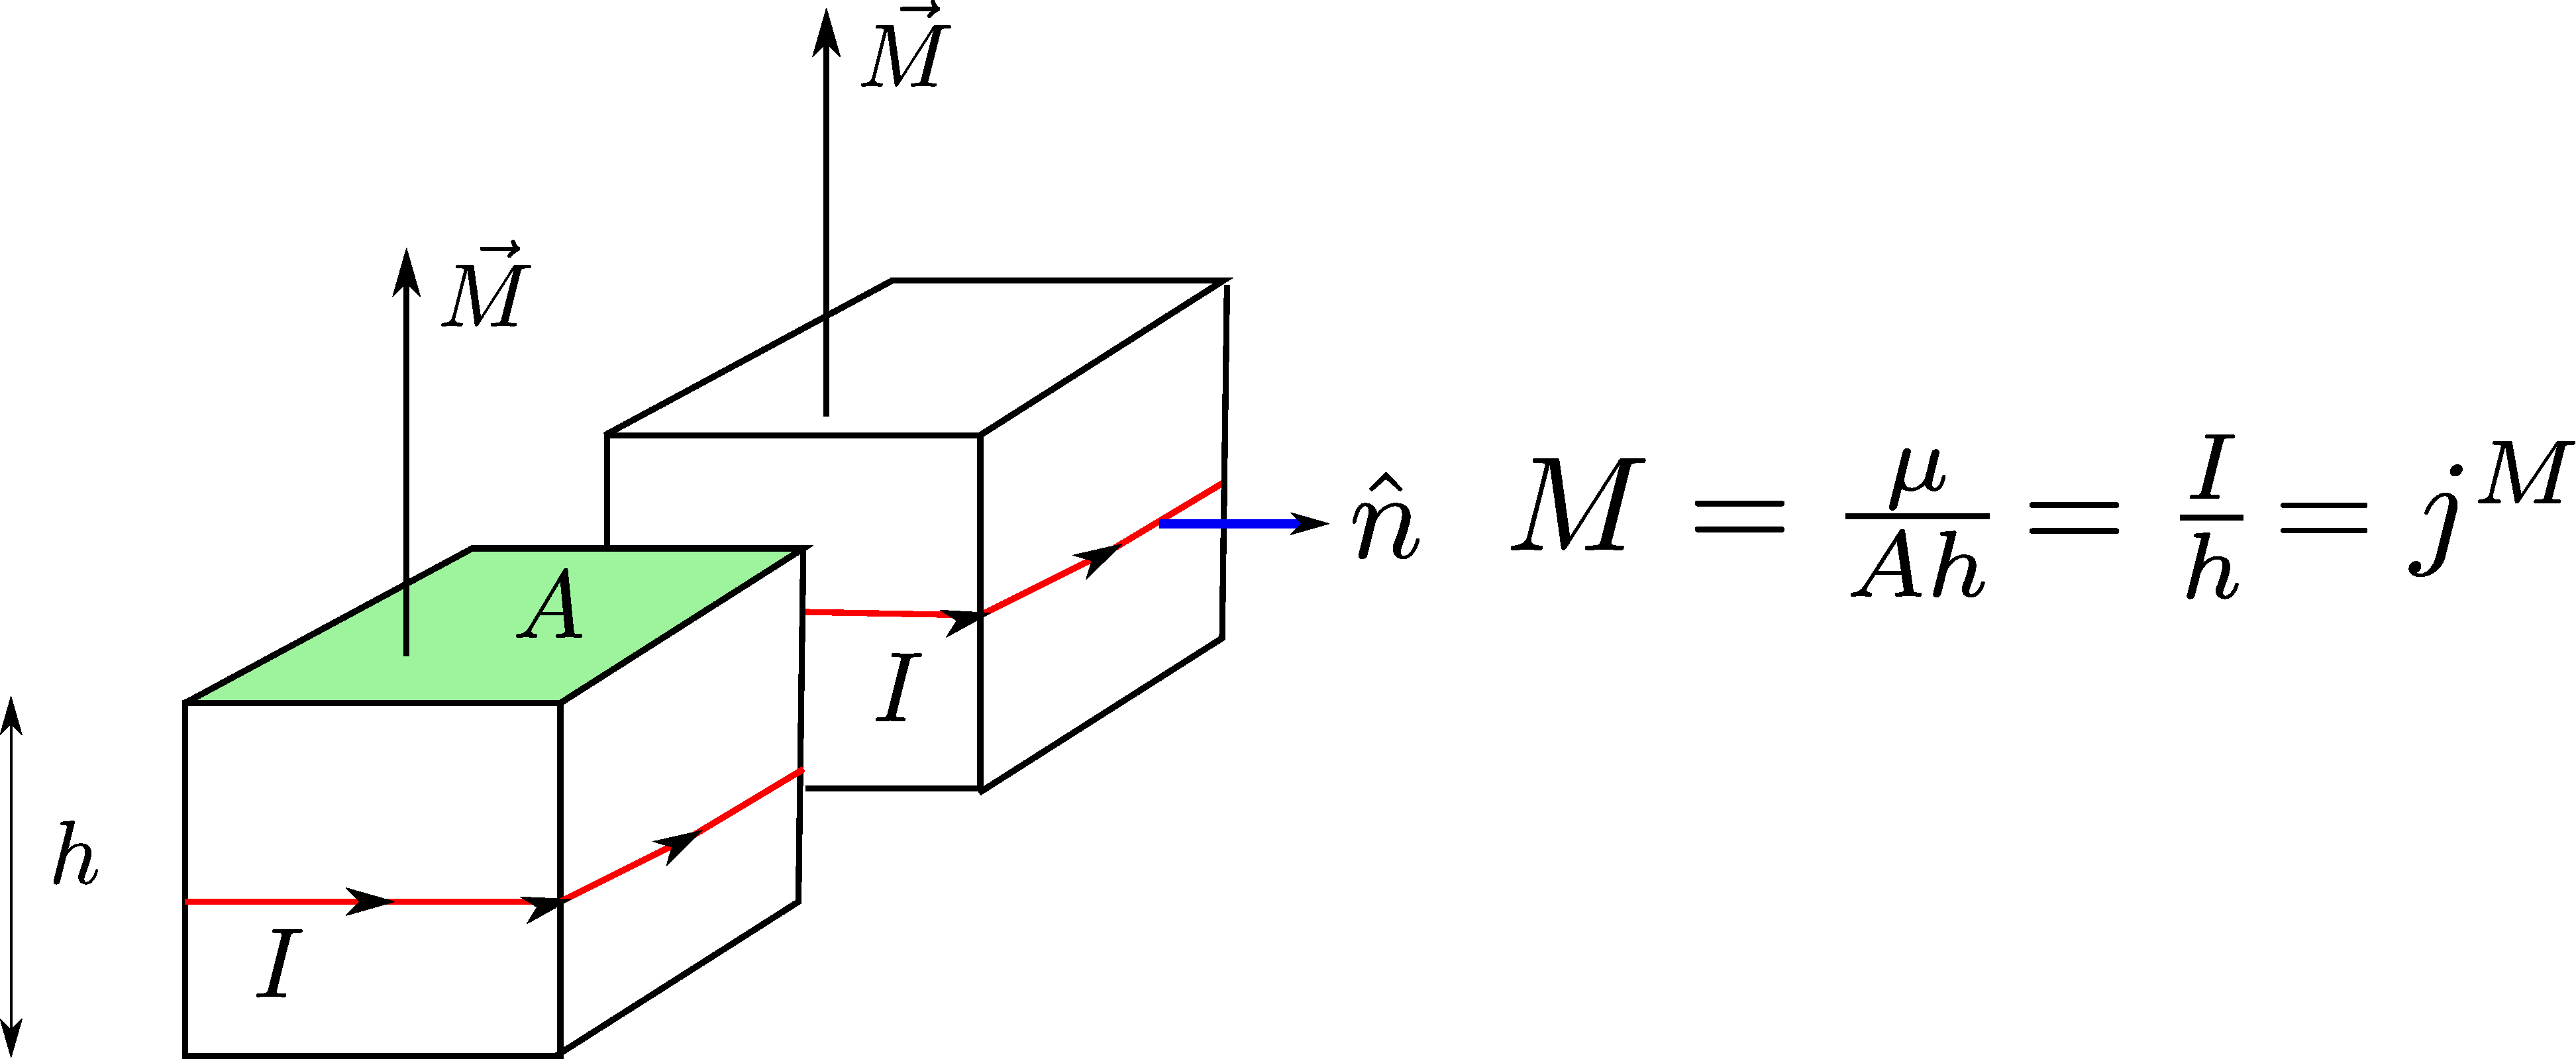
\psfig{file=fig/fig-corriente-magnetizacion-superficie.pdf,height=3cm,angle=0}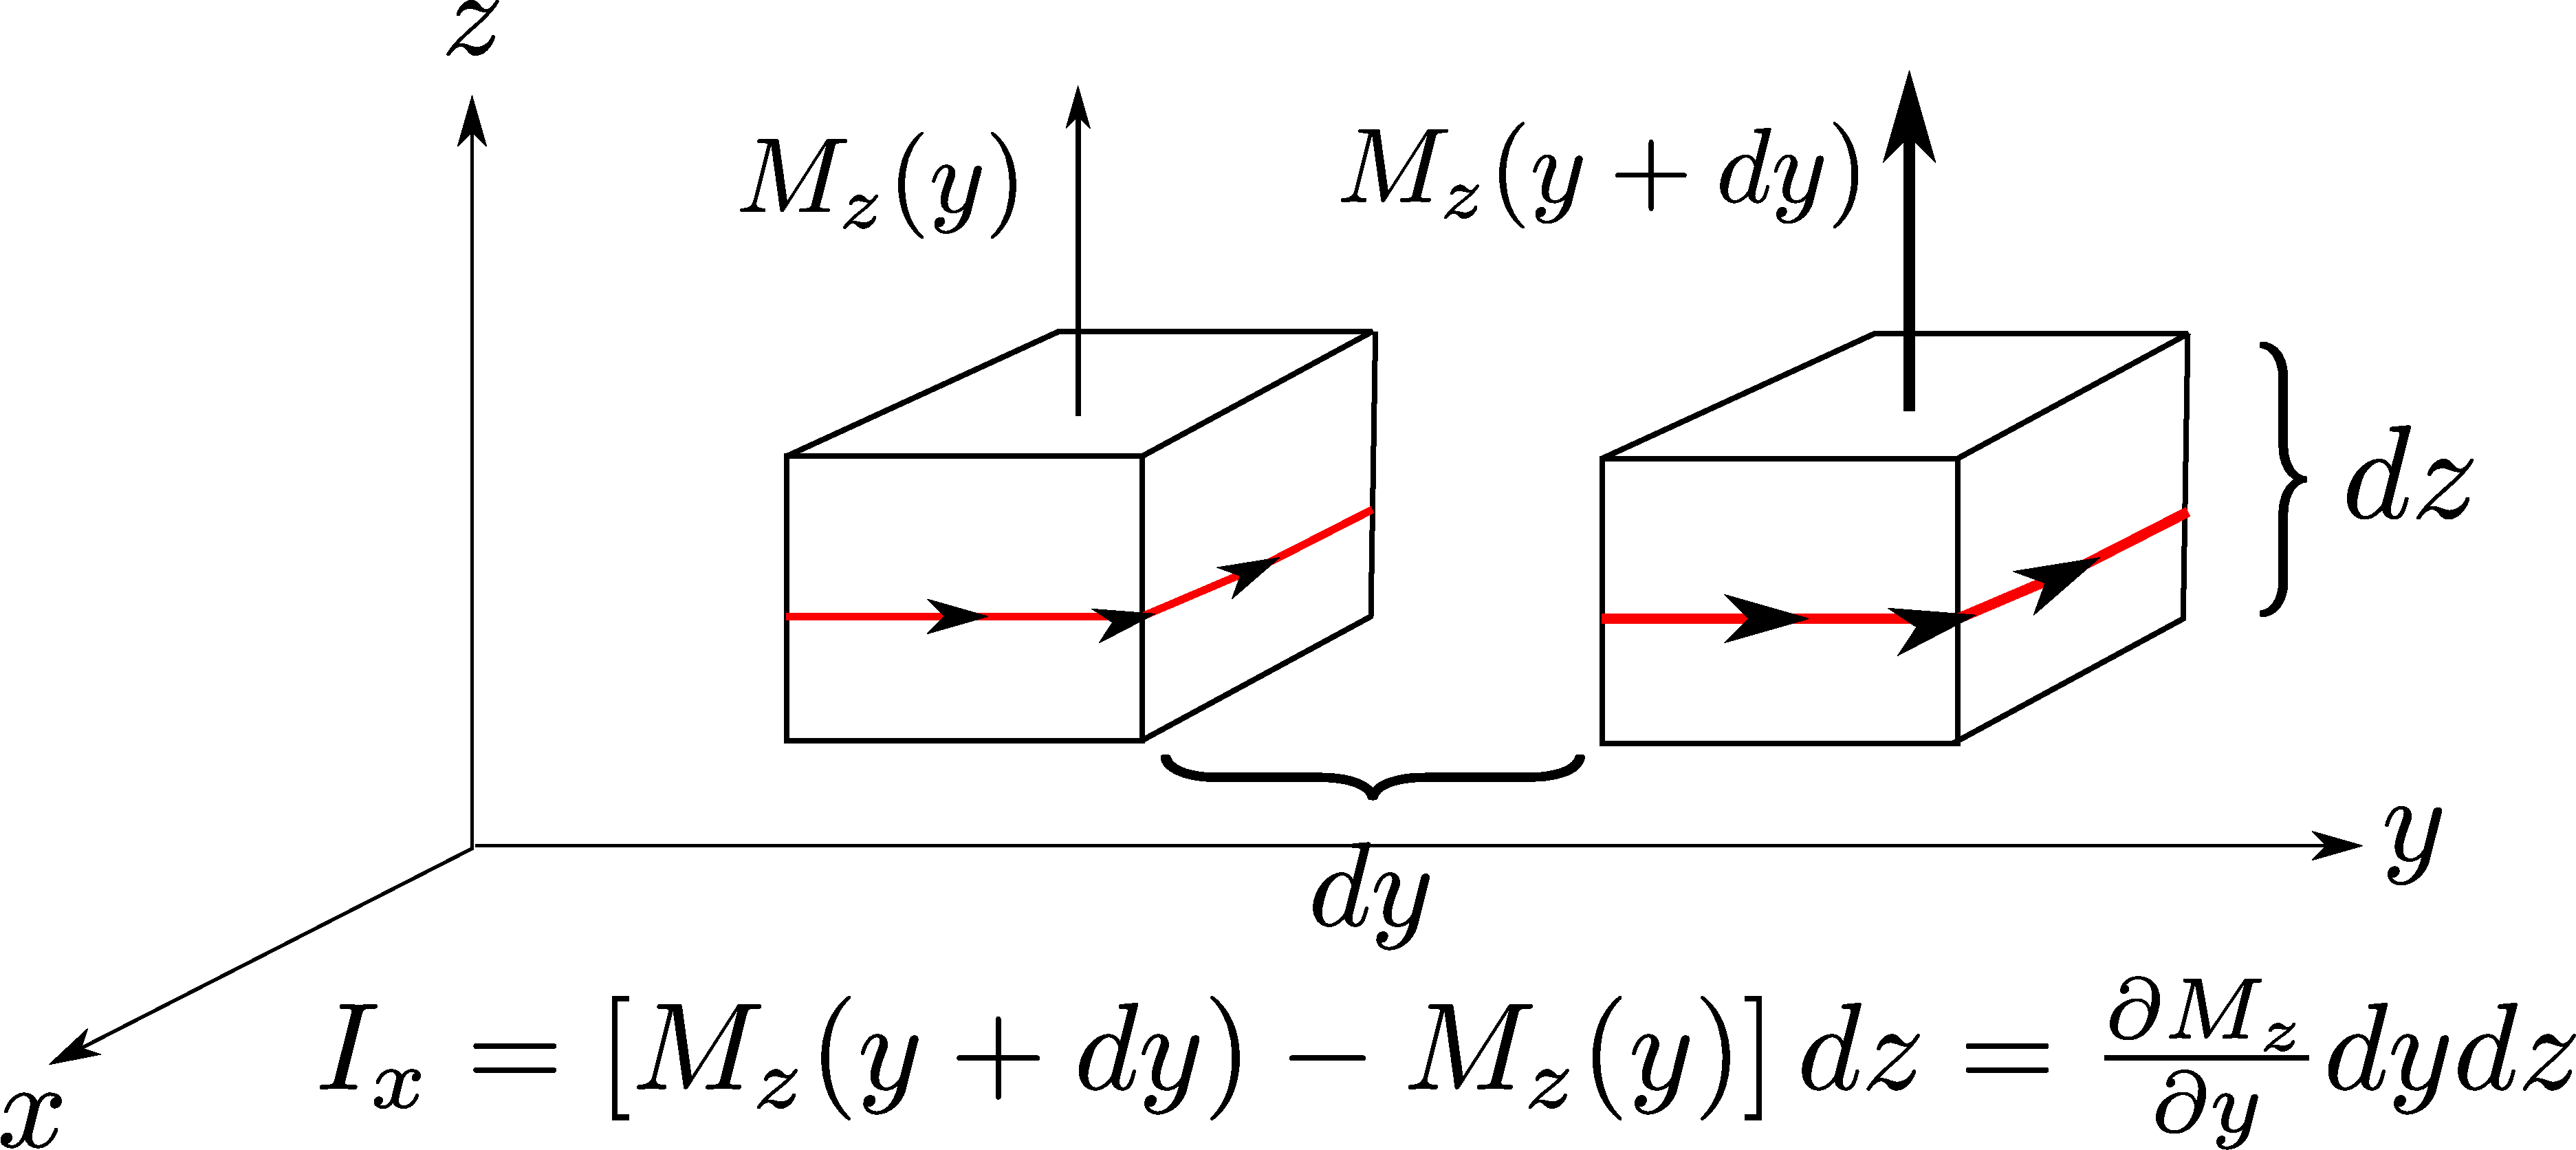
\psfig{file=fig/fig-corriente-magnetizacion-volumen.pdf,height=3cm,angle=0}}
\caption{Corrientes de magnetizaci'on de volumen y superficie. (Figura original gentileza de A. Maldonado) *** EDITAR, MEJORAR, EXPLICAR ***}
\label{fig-corriente-magnetizacion}
\end{figure}

Usando (\ref{AM1}) podemos calcular la contribuci'on de la magnetizaci'on a  la inducci'on magn'etica como:
\begin{eqnarray}
 B_i^{\rm M}&=&\varepsilon_{ijk}\partial_jA_k^{\rm M} \\
&=&\frac{\mu_0}{4\pi}\varepsilon_{ijk}\varepsilon_{kln}\int_V
M_l(x')\partial_j\partial'_n\frac{1}{\left\vert\vec{x}
-\vec{x}'\right\vert}dV'\\
&=&-\frac{\mu_0}{4\pi}\left(\delta_{il}\delta_{jn}-\delta_{in}
\delta_{jl}\right)\int_VM_l(x')\partial_j\partial_n\frac{1}{\left\vert\vec{x}
-\vec{x}'\right\vert}dV'\\
&=&\frac{\mu_0}{4\pi}\int_V\left[M_j(x')\partial_j\partial_i\frac{1}{
\left\vert\vec { x }-\vec{x}'\right\vert}-M_i(x')\partial_j\partial_j\frac{1}{
\left\vert\vec { x }-\vec{x}'\right\vert}\right]dV'\\
&=&\frac{\mu_0}{4\pi}\partial_i\left[\int_VM_j(x')\partial_j\frac{1}{
\left\vert\vec{x}-\vec{x}'\right\vert}dV'\right]-\frac{\mu_0}{4\pi}\int_V
M_i(x')\nabla^2\frac{1} {\left\vert\vec {x}-\vec{x}'\right\vert}dV'\\
&=&-\frac{\mu_0}{4\pi}\partial_i\left[\int_VM_j(x')\partial'_j\frac{1}{
\left\vert\vec{x}-\vec{x}'\right\vert}dV'\right]+\mu_0\int_V
M_i(x')\delta^{(3)}(\vec{x}-\vec{x}')dV',
\end{eqnarray}
de donde obtenemos:
\begin{equation}
 \boxed{\vec{B}^{\rm M}(x)=\mu_0\vec{M}(x)-\mu_0\vec\nabla\phi^*_{\rm M}(x),}
\label{BM}
\end{equation}
donde hemos definido el \textbf{potencial escalar de magnetizaci'on}\footnote{Note que 'este es un campo \textit{distinto} al potencial escalar magn'etico definido en la secci'on \ref{secpem}.}
\begin{equation}\marginnote{Potencial escalar de magnetizaci'on}
 \boxed{\phi^*_{\rm M}(x):=\frac{1}{4\pi}\int_VM_j(x')\partial'_j\frac{1}{
\left\vert\vec{x}-\vec{x}'\right\vert}dV'=\frac{1}{4\pi}
\int_V\frac{\vec{M}(x')\cdot (\vec{x}-\vec{x}')}{\left\vert\vec{x}-\vec{x}
'\right\vert^3} dV'. }
\end{equation}
En un sistema general existir'an, adem'as de la magnetizaci'on, corrientes
\textit{externas} (tambi'en llamadas \textit{libres} o \textit{de transporte}),
por lo que la inducci'on magn'etica total es dada por:
\begin{equation}
 \vec{B}(x)=\vec{B}^{\rm ext}(x)+\vec{B}^{\rm M}(x) .
\end{equation}
Usando (\ref{BS2}) y (\ref{BM}) encontramos finalmente una expresi'on para 
la inducci'on magn'etica macrosc'opica total en un medio magnetizado y con
corrientes externas:
\begin{equation}\marginnote{$\vec{B}$: corrientes externas + magnetizaci'on}
\boxed{ \vec{B}(x)=\frac{\mu_0}{4\pi}\int_V\frac{\vec{J}_{\rm ext}
(x')\times\left(\vec{x}-\vec{x}'\right)}{\left\vert\vec{x}-\vec{x}'\right\vert^3
} dV' +\mu_0\vec{M}(x)-\mu_0\vec\nabla\phi^*_{\rm M}(x).}
\label{BMG}
\end{equation}

\subsection{Excitaci'on magn'etica}\label{sec:defH}
Al calcular el rotor del campo definido en (\ref{BMG}), vea (\ref{ley-Ampere}),
encontramos:
\begin{equation}
 \vec\nabla\times\vec{B}=\mu_0\,\vec{J}_{\rm ext}
+\mu_0\vec\nabla\times\vec{M}.
\end{equation}
De aqu'i, podemos escribir
\begin{equation}
 \vec\nabla\times\left(\frac{1}{\mu_0}\vec{B}-\vec{M}\right)=\vec{J}_{
\rm ext}.
\end{equation}
Esto motiva definir la \textbf{excitaci'on magn'etica} (tambi'en llamada
\textbf{intensidad de campo magn'etico}):
\begin{equation}\marginnote{Excitaci'on magn'etica}\label{defH}
\boxed{\vec{H}(x):=\frac{1}{\mu_0}\vec{B}(x)-\vec{M}(x),}
\end{equation}
es decir,
\begin{equation}\label{HJM}
\vec{H}(x):=\frac{1}{4\pi}\int_V\frac{\vec{J}_{\rm ext}
(x')\times\left(\vec{x}-\vec{x}'\right)}{\left\vert\vec{x}-\vec{x}'\right\vert^3
} dV' -\vec\nabla\phi^*_{\rm M}(x) ,
\end{equation}
que satisface entonces la ``ley de Amp\`ere'',
\begin{equation}\marginnote{L. de Amp\`ere para $\vec{H}$}
 \boxed{\vec\nabla\times\vec{H}=\vec{J}_{\rm ext}} \label{rotHj}
\end{equation}
o, en su versi'on integral,
\begin{equation}
 \boxed{\oint_{\cal C}\vec{H}\cdot d\vec\ell=I_{\rm ext} .} \label{intHI}
\end{equation}
An'alogamente al caso del vector de desplazamiento el'ectrico $\vec{D}$, la
intensidad de campo magn'etico $\vec{H}$ es una cantidad 'util puesto que est'a
relacionada, a trav'es de la ecuaci'on (\ref{rotHj}), con las corrientes
externas del sistema, que son las corrientes que (en principio) pueden ser
manipuladas.

A partir de (\ref{HJM}) vemos que \textit{en regiones sin corrientes externas}, la excitaci'on magn'etica puede derivarse 'integramente del potencial escalar de magnetizaci'on\footnote{Compare con \eqref{Bgradphi}.},
\begin{equation}\marginnote{Si $\vec{J}_{\rm ext}=\vec{0}$}\label{HpM}
\vec{H}(x)= -\vec\nabla\phi^*_{\rm M}(x).
\end{equation}

\subsection{Condiciones de continuidad en interfaces}
\begin{figure}[!h]
\centerline{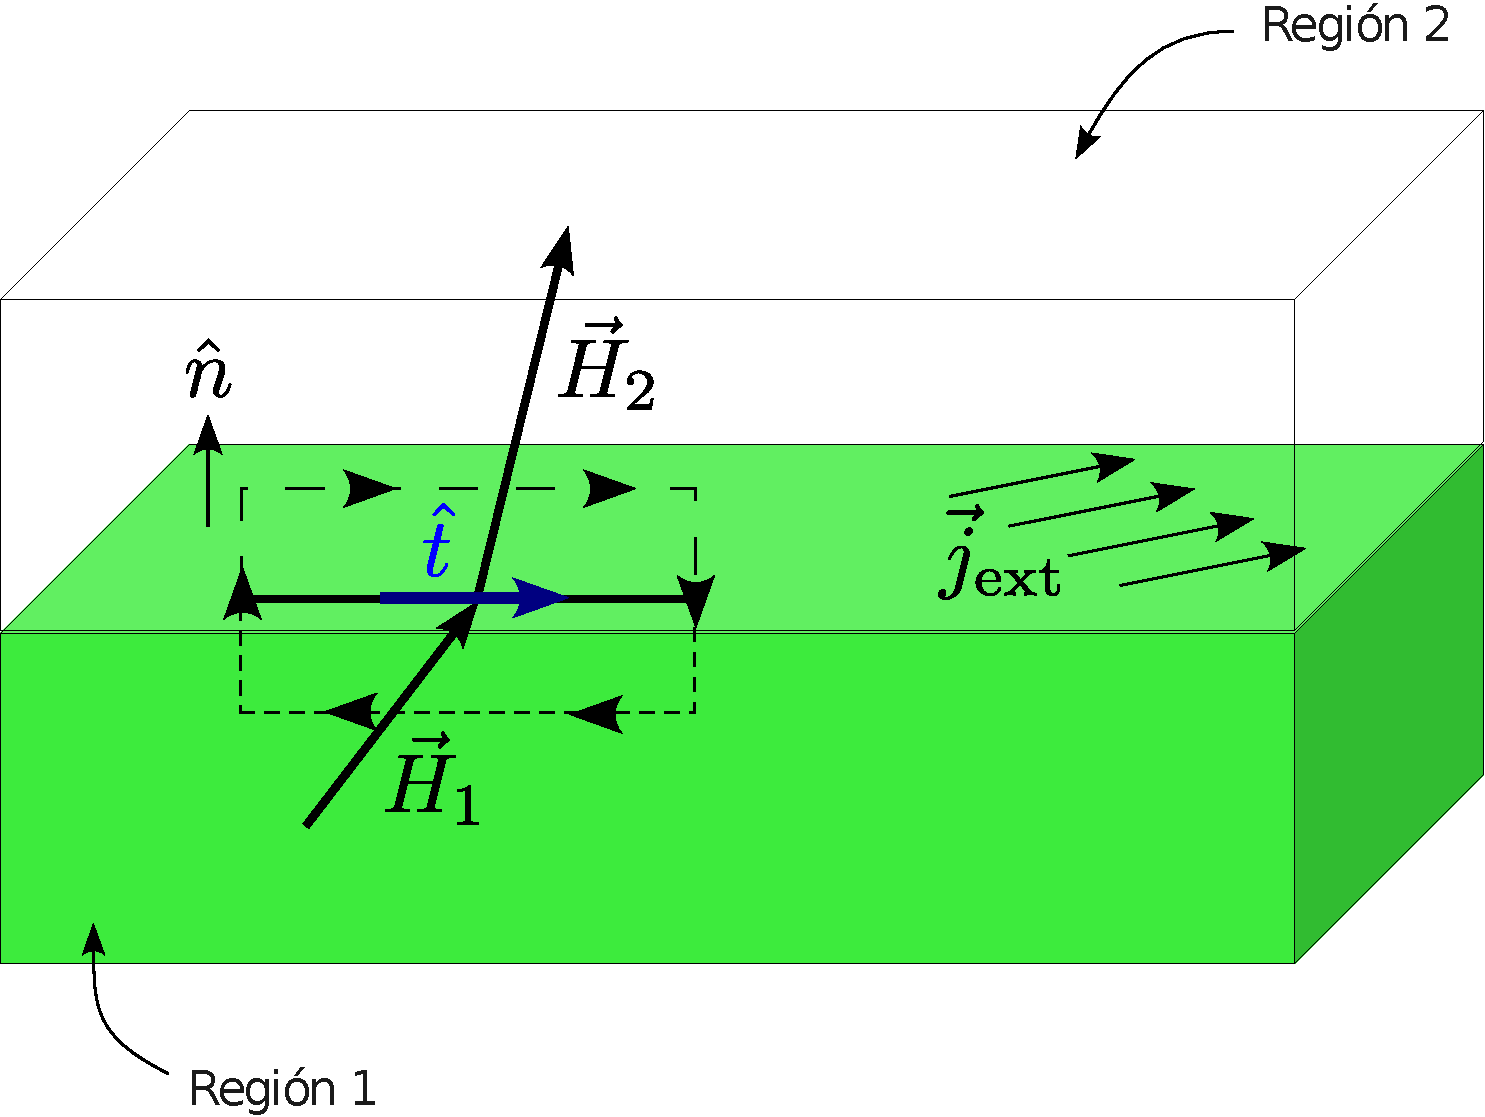
\psfig{file=fig/fig-condicion-borde-magnetica-01.pdf,height=5cm,angle=0}}
\caption{Condiciones de continuidad para $\vec{H}$ en una interface de dos
medios magn'eticos.}
\label{BM1}
\end{figure}
Al aplicar la ley de Amp\`ere (\ref{intHI}) al circuito de la figura \ref{BM1},
y considerando que
\begin{equation}\label{IextjS}
 I_{\rm ext}=\int_S\vec{J}_{\rm ext}\cdot d\vec{S}=\int_S\vec{J}_{\rm ext}\cdot
(\hat{n}\times\hat{t})\,dS=\vec{j}_{\rm ext}\cdot
(\hat{n}\times\hat{t})\,\ell=(\vec{j}_{\rm ext}\times\hat{n})\cdot\hat{t}\,\ell ,
\end{equation}
encontramos
\begin{equation}
 \boxed{\left(\vec{H}_2-\vec{H}_1\right)\cdot\hat{t}=(\vec{j}_{\rm
ext}\times\hat{n})\cdot\hat{t}} \label{Hint}
\end{equation}
o, equivalentemente
\begin{equation}
\boxed{\hat{n}\times\left(\vec{H}_2-\vec{H}_1\right)=\vec{j}_{\rm
ext}.}
\end{equation}
Note que en (\ref{IextjS}) el lado derecho contiene a la \textbf{densidad de corriente superficial externa} $\vec{j}_{\rm ext}$. En este caso puede considerarse que $\vec{J}_{\rm ext}=\vec{j}_{\rm ext}\delta(z)$, donde la superficie que limita las dos regiones est'a determinada por la condici'on $z=0$, siendo $z$ una coordenada normal a la superficie.

\textbf{Si no hay corrientes externas de superficie, entonces la componente \textit{tangencial} de la excitaci'on magn'etica cruza continuamente la interface}. En general, si
existen corrientes externas de superficie, la componente de la intensidad de
campo magn'etico paralela a $\vec{j}_{\rm ext}=j_{\rm ext}\,\hat{\jmath}$ cruzar'a continuamente la interface, mientras que la componente ortogonal tendr'a una discontinuidad de magnitud $j_{\rm ext}$. Esto puede verse directamente
de (\ref{Hint}) eligiendo $\hat{t}$ en la direcci'on y sentido de
$\vec{j}_{\rm ext}$, es decir, $\hat{t}=\hat{\jmath}$, obteniendo
\begin{equation}
 H_2^\parallel=H_1^\parallel,  \qquad H^\parallel:=\vec{H}\cdot\hat{\jmath},
\end{equation}
mientras que, eligiendo $\hat{t}=\hat{\jmath}\times\hat{n}$, encontramos
\begin{equation}
 H_2^\perp-H_1^\perp=j_{ext},  \qquad
H^\perp:=\vec{H}\cdot(\hat{\jmath}\times\hat{n}).
\end{equation}

Estas relaciones se complementan con aquella que se desprende del hecho que el campo magn'etico tiene siempre divergencia nula (independientemente del medio considerado). An'alogamente al caso el'ectrico, ver por ejemplo \eqref{saltoDn}, la ecuaci'on \eqref{divB} implica 
\begin{equation}\label{saltoBn}
\boxed{\left(\vec{B_2}-\vec{B_1}\right)\cdot\hat{n}=0,}
\end{equation}
es decir, la componente de $\vec{B}$ normal a la superficie es continua en la interface.

\subsection{Relaci'on constitutiva, susceptibilidad magn'etica}
An'alogamente al caso electrost'atico, se llama relaci'on constitutiva a la
relaci'on entre la magnetizaci'on de un material (la ``respuesta'' de 'este)
con el campo magn'etico existente, por ejemplo:
\begin{equation}
 \vec{M}=\vec{M}[\vec{H}].
\end{equation}
Esta relaci'on puede ser no-local, no-lineal, anis'otropa e inhomog'enea, y es usualmente inferida a partir de experimentos. Sin
embargo, muchos materiales pueden ser descritos por relaciones \textit{locales}. En
este caso puede parametrizarse la dependencia de la magnetizaci'on con la
intensidad magn'etica por medio de una serie de la forma
\begin{equation}
M_i(x)=M_i(H_j(x))=\left.M_i\right|_{\vec{H}=\vec{0}}
+\chi^{\rm m}_{ij}(x)H_j(x)+\chi^{\rm m}_{ijk}(x)H_j(x)H_k(x)+\cdots.
\end{equation}
%\begin{equation}
%M_i(x)=M_i(H_j(x))=\left.M_i\right|_{\vec{H}=\vec{0}}
%+H_j\left(\partial_jM_i\right)_{\vec{H}=\vec{0}}+\frac{1}{2}
%H_jH_k\left(\partial_j\partial_k M_i\right)_{\vec{H}=\vec{0}}+\cdots.
%\end{equation}
Para medios locales, \textit{lineales} y \textit{sin magnetizaci'on permanente}
($\left.M_i\right|_{\vec{H}=\vec{0}}=0$), la relaci'on se reduce a
\begin{equation}
 \boxed{M_i(x)=\chi^{\rm m}_{ij}(x)H_j(x),}
\end{equation}
donde $\chi^{\rm m}_{ij}$ es el \textbf{tensor de susceptibilidad magn'etica} del
material. En este caso, la inducci'on magn'etica adopta la forma
\begin{equation}
 \boxed{B_i(x)=\mu_{ij}(x)H_j(x)=\mu_0\,\kappa^{\rm m}_{ij}(x)H_j(x),}
\end{equation}
con el tensor de \textbf{permeabilidad magn'etica} $\mu_{ij}$ y el
tensor de \textbf{permeabilidad relativa} $\kappa^{\rm m}_{ij}$, definidos por
\begin{equation}
 \boxed{\mu_{ij}:=\mu_0\left(\delta_{ij}+\chi^{\rm
m}_{ij}\right)=\mu_0\kappa^{\rm m}_{ij}.}
\end{equation}
Finalmente, en el caso de medios locales, lineales e is'otropos, las
expresiones anteriores para la relaci'on constitutiva se reducen a
\begin{equation}
 \vec{M}(x)=\chi_{\rm m}(x)\vec{H}(x),
\end{equation}
\begin{equation}
 \vec{B}(x)=\mu(x)\vec{H}(x)=\mu_0\,\kappa_{\rm m}(x)\vec{H}(x),
\end{equation}
\begin{equation}
 \mu:=\mu_0\left(1+\chi_{\rm m}\right)=\mu_0\kappa_{\rm m}.
\end{equation}


\subsubsection{Ecuaci'on de Laplace para el potencial escalar de magnetizaci'on}
Como vimos en la secci'on \ref{sec:defH}, \textit{en regiones libres de corrientes externas} la excitaci'on magn'etica $\vec{H}$ es propocional al gradiente del potencial escalar de magnetizaci'on, ver (\ref{HpM}). Si adem'as el medio es \textit{lineal e is'otropo}, entonces $\vec{B}=\mu\vec{H}=-\mu\vec{\nabla}\phi^\ast_{\rm M}$. Finalmente, si adem'as el medio es \textit{homog'eneo}, encontramos, usando (\ref{divB}), que el potencial escalar de magnetizaci'on satisface la ecuaci'on de Laplace,
\begin{equation}
\nabla^2\phi^\ast_{\rm M}=0.
\end{equation}


\subsection{Paramagnetismo, diamagnetismo, ferromagnetismo}

\subsubsection{Diamagnetismo}
En este tipo de materiales $\vec{M}$ \textbf{tiene direcci'on opuesta a}  $\vec{H}$, por lo que $\chi_{\rm m}<0$ y $\kappa_{\rm m}<1$ y la inducci'on magn'etica $\vec{B}$ es \textbf{debilidata} (respecto al valor que asumir'ia en el vac'io, dada la misma distribuci'on de corrientes externas). Este tipo de materiales requiere que no existan \textit{momentos magn'eticos permanentes} significativos, de modo que la magnetizaci'on se deba principalmente a \textbf{corrientes inducidas}. Estas \textbf{corrientes inducidas generan momentos dipolares en sentido contrario al campo que las induce}, por lo que \textbf{la inducci'on magn'etica disminuye en el interior de un diamagneto}. En la mayor'ia de los casos de diamagnetismo la susceptibilidad magn'etica es independiente de la
temperatura y posee un valor muy peque\~no: $|\chi_{\rm m}|\lesssim 10^{-5}$. El
diamagnetismo es una propiedad general, es decir, que se presenta en todos los
materiales (siempre se producen peque\~nas corrientes inducidas), pero se dice
que un material es diamagn'etico si este efecto es el dominante, es decir,
cuando no existen otras fuentes de magnetizaci'on que reviertan la contribuci'on diamagn'etica.
Ejemplos de materiales diamagn'eticos: casi todas las substancias org'anicas,
metales nobles (oro, plata, cobre, mercurio, ...). Un caso extremo de
diamagnetismo es un \textbf{superconductor}, en el que la inducci'on magn'etica
es \textbf{anulada en su interior}, $\chi_{\rm m}=-1$ y $\kappa_{\rm m}=0$ (``diamagneto ideal'').

\subsubsection{Paramagnetismo}
 En este tipo de materiales la magnetizaci'on $\vec{M}$
tiene la misma direcci'on y sentido que $\vec{H}$. Equivalentemente $\vec{M}$
tiene la misma direcci'on y sentido que $\vec{B}$, de modo que
$\chi_{\rm m}>0$, $\kappa_{\rm m}>1$. Por esto, en un material paramagn'etico la inducci'on magn'etica $\vec{B}$ es \textbf{reforzada}. Este caso requiere que el material posea \textit{momentos magn'eticos permanentes}, que puedan anilearse con el campo magn'etico.
A la tendencia de los momentos magn'eticos a alinearse se
contrapone el ``desorden'' relacionado con las agitaciones t'ermicas del
material. Por esto, \textbf{en un material paramagn'etico $\chi_{\rm}$ disminuye a
medida que la temperatura aumenta}. Muchos materiales paramagn'eticos satisfacen
la \textbf{ley de Curie}: $\chi_{\rm}\propto 1/T$.
\begin{table}[h!]
\begin{center}
\begin{tabular}{c|c}
Material & $\chi_{\rm m}$ \\ \hline\hline
Aluminio & $2,1\times 10^{-5}$ \\
Cobre & $-0,98\times 10^{-5}$ \\
Oro & $-3,5\times 10^{-5}$ \\
Magnesio & $1.2\times 10^{-5}$ \\
Mercurio & $-2,8\times 10^{-5}$ \\
Plata & $-2,4\times 10^{-5}$ \\
Sodio & $0.84\times 10^{-5}$ \\
Titanio & $18.0\times 10^{-5}$ \\
Tungsteno & $7.6\times 10^{-5}$ \\
Hidr'ogeno (1 atm) & $-0,22\times 10^{-8}$ \\
Nitr'ogeno (1 atm) & $-0,67\times 10^{-8}$ \\
Ox'igeno (1 atm) & $193,5\times 10^{-8}$
\end{tabular}
\caption{Algunos materiales y sus susceptibilidades magn'eticas, a temperatura ambiente (Reitz-Milford).}
\end{center}
\end{table}

\subsubsection{Ferromagnetismo}

 En este tipo de materiales (t'ipicamente materiales que
contienen Fierro, Cobalto o N'iquel) \textbf{la magnetizaci'on no es
proporcional a la excitaci'on magn'etica}. Esto es algunas veces expresado
diciendo que la \textbf{susceptibilidad magn'etica efectiva} $\chi_{\rm m}:=M/H$ depende del valor del campo (y de otras variables, como por ejemplo de la temperatura), $\chi_{\rm m}=\chi_{\rm m}(T,\vec{H})$. El ferromagnetismo
requiere tambi'en que el material posea dipolos magn'eticos permanentes. Debido
a interacciones cu'anticas, los momentos magn'eticos de un ferromagneto se
ordenan \textit{espont'aneamente} (es decir, sin necesidad de campo magn'etico
externo), cuando la temperatura baja de un cierto valor cr'itico, llamada
temperatura de Curie, $T_{\rm C}$. En el cero absoluto de temperatura, todos los
momentos magn'eticos estar'ian alineados. A medida que la temperatura aumenta, el
desorden inducido por las vibraciones t'ermicas tiende a disminuir la
alineaci'on, pero sin conseguir
anular la magnetizaci'on total. Cuando la temperatura cruza la temperatura de
Curie, el sistema experimenta una transici'on de fase, y a partir de ese
momento se comporta como un paramagneto usual.
\begin{table}[h!]
\begin{center}
\begin{tabular}{c||c|c|c|c|c|c}
Material & Fe & Co & Ni & Gd & EuO & CrBr${}_3$  \\ \hline
$T_{\rm C}$ [K] & 1043 & 1393 & 631 & 290 & 69 & 37
\end{tabular}
\caption{Algunos materiales ferromagn'eticos y sus temperaturas de Curie 
\cite{Nolting}.}
\end{center}
\end{table}

T'ipicamente, los ferromagnetos poseen susceptibilidades
magn'eticas muy altas y \textbf{la magnetizaci'on que presentan depende de
su historia}, es decir, de c'omo hayan sido expuestos a campos externos. En
otras palabras, \textbf{dado un valor de la excitaci'on $\vec{H}$ el valor de $\vec{M}$
no es 'unico, sino que depende de c'omo se haya alcanzado el valor $\vec{H}$}.
Este fen'omeno es conocido como \textbf{hist'eresis}. El comportamiento de
hist'eresis t'ipico de un ferromagneto es ilustrado en la figura
\ref{fig-histeresis}.
\begin{figure}[!h]
\centerline{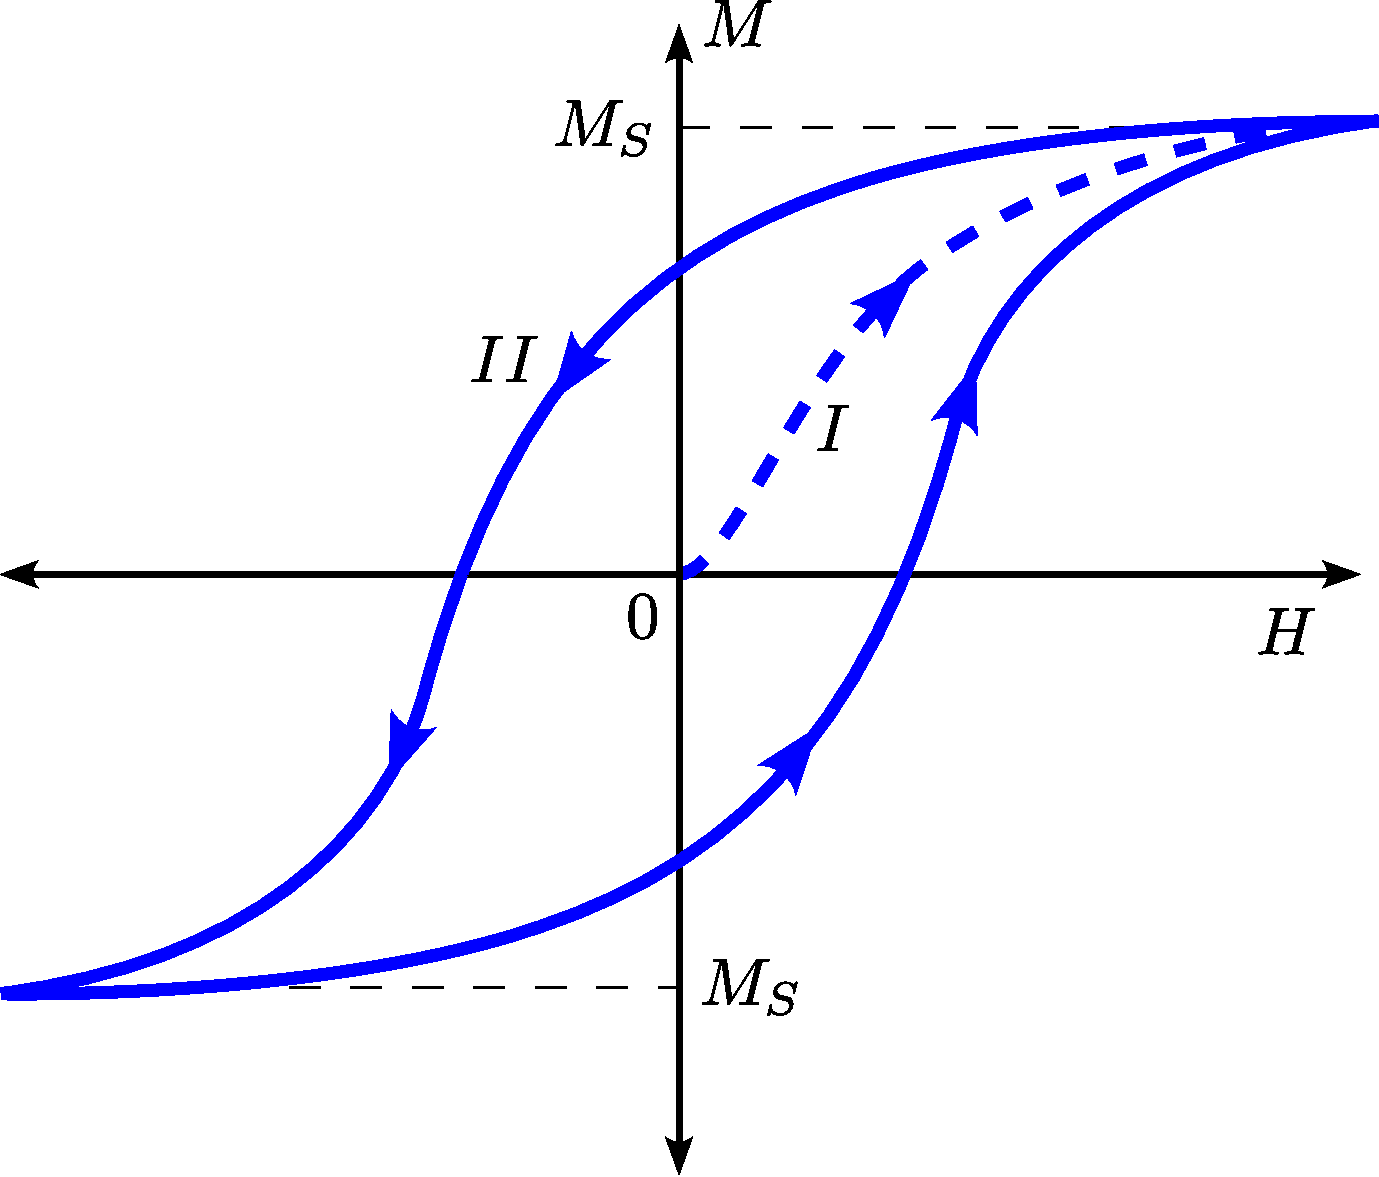
\psfig{file=fig/fig-histeresis-01.pdf,height=6cm,angle=0}}
\caption{Curva de hist'eresis t'ipica para un material ferromagn'etico.}
\label{fig-histeresis}
\end{figure}
Un material ferromagn'etico sin magnetizaci'on previa sometido a un campo $H$
se magnetiza siguiendo la curva I, llegando a una magnetizaci'on m'axima $M_S$ (``magnetizaci'on de saturaci'on"). 
Si luego se disminuye la intensidad de campo magn'etico el sistema se comienza
a demagnetizar, pero siguiendo la curva II, de modo que, incluso cuando el
campo $H$ es cero, el material conserva una magnetizaci'on no nula (magneto
permanente), llamada ``magnetizaci'on remanente''. Esta magnetizaci'on puede
ser anulada aplicando un campo en sentido inverso (intensidad de campo
``coercitivo''). La propiedad de hist'eresis est'a relacionada con la existencia
de \textbf{dominios magn'eticos}, que poseen un momento magn'etico macrosc'opico
no nulo y que requieren de energ'ia para reorientarse. La hist'eresis de los
ferromagnetos es usada en la fabricaci'on de \textbf{dispositivos de memoria}, en los
que la informaci'on es codificada en la orientaci'on del momento magn'etico de
los dominios, que permanece indefinidamente hasta que campos externos sean
usados para cambiar su estado.